% TEMPLATE for Usenix papers, specifically to meet requirements of
%  USENIX '05
% originally a template for producing IEEE-format articles using LaTeX.
%   written by Matthew Ward, CS Department, Worcester Polytechnic Institute.
% adapted by David Beazley for his excellent SWIG paper in Proceedings,
%   Tcl 96
% turned into a smartass generic template by De Clarke, with thanks to
%   both the above pioneers
% use at your own risk.  Complaints to /dev/null.
% make it two column with no page numbering, default is 10 point

% Munged by Fred Douglis <douglis@research.att.com> 10/97 to separate
% the .sty file from the LaTeX source template, so that people can
% more easily include the .sty file into an existing document.  Also
% changed to more closely follow the style guidelines as represented
% by the Word sample file. 

% Note that since 2010, USENIX does not require endnotes. If you want
% foot of page notes, don't include the endnotes package in the 
% usepackage command, below.

% This version uses the latex2e styles, not the very ancient 2.09 stuff.
\documentclass[letterpaper,twocolumn,10pt]{article}
\usepackage{usenix2019,epsfig,endnotes}
\usepackage{bm}
\usepackage{url}
\usepackage{amsmath}
\usepackage{subfig}
\usepackage{algorithm} 
\usepackage{booktabs}
\usepackage{multirow}
\usepackage{epstopdf}
\usepackage{hyperref}
\usepackage{amsfonts}
\usepackage{algpseudocode}
\begin{document}

%don't want date printed
\date{}

%make title bold and 14 pt font (Latex default is non-bold, 16 pt)
\title{\Large \bf Perceived Quality driven VR Streaming}

%for single author (just remove % characters)
\author{
{\rm Your N.\ Here}\\
Your Institution
\and
{\rm Second Name}\\
Second Institution
% copy the following lines to add more authors
% \and
% {\rm Name}\\
%Name Institution
} % end author

\maketitle

% Use the following at camera-ready time to suppress page numbers.
% Comment it out when you first submit the paper for review.
\thispagestyle{empty}


\subsection*{Abstract}
In recent years, Virtual Reality (VR) video streaming becomes popular quickly. How to provide high user-perceived quality with limited bandwidth becomes the biggest problem in VR video streaming. Traditional viewpoint-driven VR streaming makes the assumption that perceived quality is only related to viewpoint-object distance, so it simply allocates high bitrate to objects near user's viewpoint. However, In this paper we prove that user perceived quality is not only related to viewpoint-object distance, it is also related to background luminance, texture complexity, viewpoint moving speed and Depth-of-Field. With consideration of these insights, we can save x\% bandwidth while providing the same perceived quality.

To build our PQVRS, we build a model to measure perceived quality in VR display, and design an object-based tiling scheme to cut video into several tiles which can be independently encoded / decoded. Then we present our method to enable client-side perceived quality computation and optimization. We implement a prototype of PQVRS and compare its performance with state-of-art VR streaming schemes. Experimental results show that proposed PQVRS saves x\% bandwidth without decrease of perceived quality.


\section{Introduction}

In recent years, the world is becoming more virtual than we ever thought it would be. Many video service providers, such as YouTube, roll out Virtual Reality (VR) videos which provide immersive experience to users. While consuming VR videos, users can change their viewpoint, resulting in an interactive experience than consuming traditional videos with a fixed viewing direction. However, VR videos' high demand of resolution and bitrates hinder their wide spread over the Internet. How to provide high user-perceived quality with limited bandwidth becomes the biggest problem in VR video streaming.

Viewpoint-adaptive streaming is regarded as a promising way to solve the problem. It assumes that a object's user-perceived quality depends on the distance from it to user's viewpoint\cite{distance}. It allocates high bit-rate for objects near user's viewport, and allocates low bit-rate for objects far from user's viewport. 

However, viewpoint-adaptive streaming is a very coarse approximation of user-perceived quality, since user-perceived quality is not only related to object-viewpoint distance. Many prior works state that it is related to some human visual characteristics, such as luminance\cite{PSPNR}, \cite{luminance1}, texture complexity\cite{PSPNR}. We model these visual characteristics into our potential improvement evaluation, and result shows that we can save 30\% bandwidth without decrease of user perceived quality. Moreover, our user study shows that in VR video display, user-perceived quality is also related to viewpoint moving speed and Depth-of-Field (DoF). When we take consideration of these visual characteristics, we can further save 20\% bandwidth without decrease of user perceived quality.

Although these insights about user-perceived quality give us promising potential improvement, optimizing perceived quality in real VR streaming system is challenging in three aspects:

\begin{itemize}

\item \textbf{Challenge 1: Traditional Human Visual System (HVS) models can not measure perceived quality in VR video display.} Perceived quality can be well-measured in traditional video display by modeling human visual system. However, perceived quality in VR display is very different from traditional video display. So current models can not be applied. We need to build a new model to quantify perceived quality in VR display.

\item \textbf{Challenge 2: Traditional grid-like video tiling scheme performs poorly in perceived quality optimization.} To allocate different bitrate to different objects, we need to cut the video into several spatial tiles which can be independently encoded / decoded. In traditional grid-like tiling scheme, videos are cut into m*n rectangular tiles of equal size. However, in a coarse-grained tiling, performance of quality allocation is poor. In a fine-grained tiling, serious bitrate efficiency problem occurs in video encoding. Both of them make the performance of perceived quality optimization far from the optimal value.

\item \textbf{Challenge 3: Information needed for perceived quality computation is disparted on server-side and client-side.} Perceived quality depends on both video content and user behavior, so it can not be pre-computed as some traditional quality metrics (such as PSNR, MSE, SSE). Client needs to compute the perceived quality of each bitrate allocation and then make decision in realtime. However, to get information of video content with current DASH, client has to pre-request the information of each pixel from server. This communication overload even exceed the overload of actual video streaming.

\end{itemize}

In this work, we address technical challenges above, then present the design and implementation of Perceived Quality driven VR Streaming (PQVRS). PQVRS is built on three key insights:

\begin{itemize}

\item \emph{Perceived quality model in VR display can be built by simply adding several new factors on traditional perceived quality model.} Although there are several new factors which influence perceived quality in VR display, and the correlation between them may be complex, we find that their influence to perceived quality can be considered independently. So we only need to measure the perceived quality due to each of new insights, and then add them to current perceived quality model.

\item \emph{Video tiling strategy can be optimized on server side.} Since traditional grid-like tiling method fail to exactly catch objects in videos, it limits the performance of perceived quality driven rate allocation. Tiling video by objects can solve this problem. Moreover, information of objects is only related to videos, object-based tiling can be completed in advance on server-side.

\item \emph{Perceived quality computation can be decoupled.} Although server has no information about user behavior, it can still compute perceived quality with each possible user behavior situations offline. Then server sends the results to client, client combine the computation result and actual user behavior to obtain final perceived quality.

\end{itemize}

Although accurately computing perceived quality needs the value of each pixel of each frame, it can be well-approximated on client-side using much less information.

Taken together, these insights enable us to engineer a Perceived Quality driven VR Streaming (PQVRS). In PQVRS, we decouple the visual characteristics due to video objects and user viewpoint, and build the VR streaming system which consider visual characteristics of video objects completely on server-side, and considers visual characteristics of user viewpoint pattern completely on client-side.

We implemented a prototype of PQVRS. We ran a pilot study on one content provider with x sessions. Our experiments show that PQVRS can save 45\% bandwidth compared with state-of-art VR streaming solutions, without decrease of perceived quality. In real-world adaptive streaming with unstable throughput, we obtain significantly higher user-perceived quality without introducing stalling. (Fig. \ref{first_image})

    \begin{figure}
  \centering
  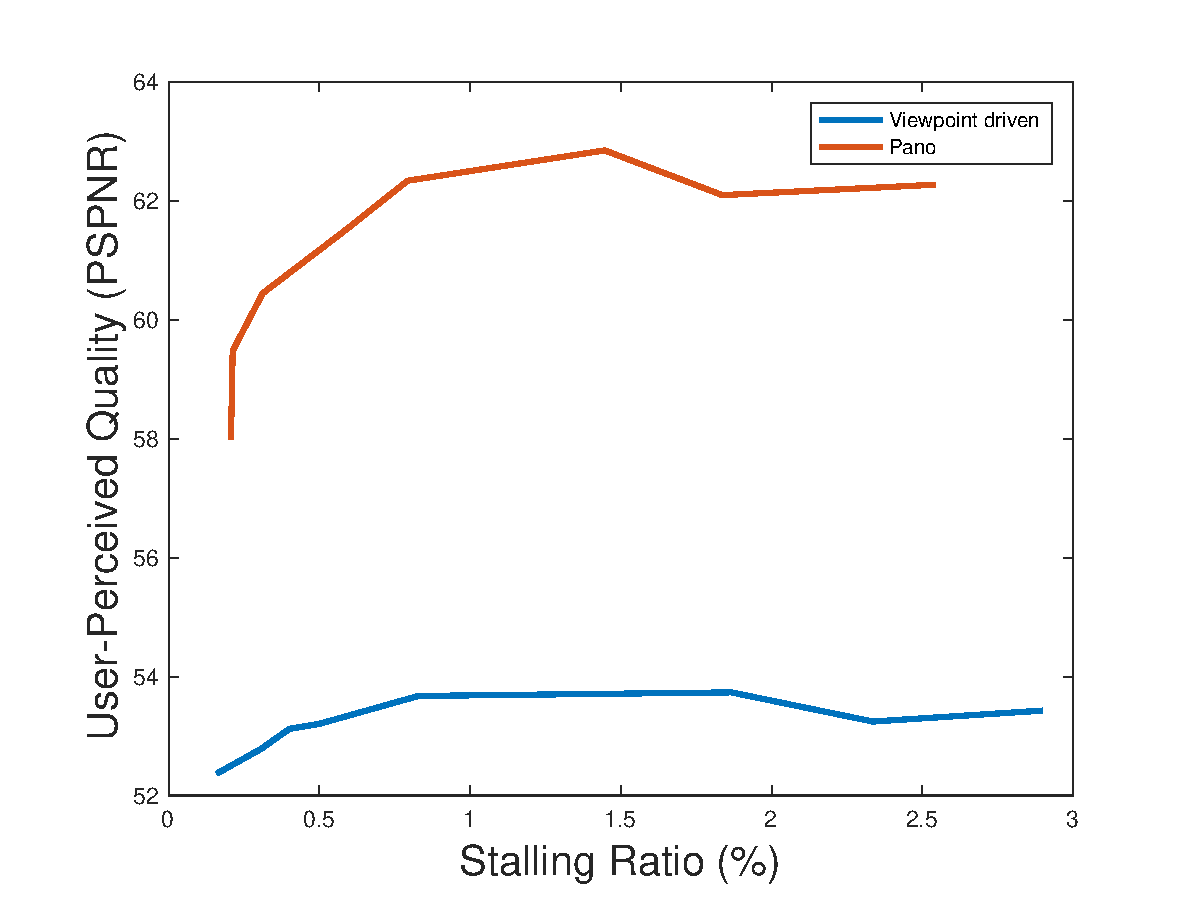
\includegraphics[width=3in]{images/first_image.eps}
  \caption{Performance comparison of Pano v.s. traditional viewpoint-driven video streaming under average throughput of 1Mbps, with bandwidth fluctuation. Each plot indicates a video session. We present 75\% ellipse confidence area.}
  \label{first_image}
  \end{figure}

\textbf{Contributions and Roadmap:}
\begin{itemize}
\item Identifying key visual characteristics which influence user-perceived quality in VR display and estimate potential improvement for it. (\S 2)
\item Identifying key challenges of building a practical perceived-quality-driven VR video streaming system and present our solutions. (\S 3-6)
\item Real-world evaluation that demonstrates substantial performance improvement by PQVRS (\S 7-8).
\end{itemize}

\section{Motivation}

In the field of psychology and biology, it is widely accepted that in a video display, user-perceived quality is very different from original video quality. It is mainly caused by human visual system \cite{contrast_masking} \cite{letter} and human brain signal processing system \cite{brain}.

In this section we show that current rate allocation strategies in VR streaming is far from optimizing user-perceived quality. If we can rightly allocate bitrate for each part of video to maximize user-perceived quality, we can save 50\% bandwidth in the same user-perceived quality, compared with state-of-art methods.

\subsection{Current VR streaming solutions}

In this section we briefly introduce two widely-used VR streaming solutions: monolithic streaming and viewport-driven streaming.

\subsubsection{Monolithic streaming}

Monolithic streaming is a widely used scheme in many VR video providers (e.g. IQiyi, Youku, ...). In monolithic streaming, it is assumed that user-perceived quality is rightly equal to video quality. A VR video is considered the same as a traditional non-VR video, so each spatial part of video is allocated to one same bitrate level. Client chooses a proper bitrate for the whole video chunk according to bandwidth throughput, buffer or other factors.

Monolithic streaming's biggest advantage is easy deployment. Since it deliveries VR video as non-VR video, there is no need to change the video streaming protocol. It can be directly applied on current video streaming system.

The disadvantage of monolithic streaming is obvious. Since in a VR video display, most area of video is out of user's viewport, which are absolutely not viewed by user. Monolithic streaming allocate the same quality level for both in-viewport part and out-viewport part. So it causes serious waste of bandwidth. 

\subsubsection{Viewpoint-driven streaming}
Many user studies have proved that perceived quality of an object in a video is highly related to its distance to user viewpoint. When an object is near to user viewpoint, it should be allocated high bitrate since user is sensitive to its distortion. When an object is far from user viewpoint, it should be allocated low bitrate since distortion is difficult to be noticed.

Viewpoint-driven streaming (\cite{viewpoint-driven1}, \cite{viewpoint-driven2}, \cite{viewpoint-driven3}, \cite{viewpoint-driven4}, \cite{viewpoint-driven5}, \cite{viewpoint-driven6}, \cite{Flare}) allocates bitrate for each object in a video based on its distance to user viewpoint. Video is usually cut into several spatial tiles, which can be independently encoded / decoded. Then it can decide the bitrate in tile-level granularity.

In addition, viewpoint prediction technology is needed in viewpoint-driven streaming, since we need to predict user's viewpoint in the next few seconds. Fortunately, in recent years, viewpoint prediction have been well studied and many solutions can obtain high prediction accuracy (\cite{viewpoint-driven1}, \cite{VPprediction}, \cite{Flare}).

Compared with monolithic streaming, viewpoint-driven streaming can allocate more bitrate for area near the user's viewpoint so it can save a lot of bandwidth while maintaining the same user-perceived quality.

\subsection{What influences user-perceived quality}
In viewpoint-driven streaming, there is a strong assumption that user-perceived quality is only related to viewpoint-object distance. Although viewpoint-driven streaming saves much bandwidth compared with monolithic streaming, it is still far away from user-perceived quality optimization.

In fact, in a video display, user-perceived quality is also related to many other factors:

\begin{itemize}

\item \emph{Perceived quality is highly related to content luminance.} For a very dark content or a very bright content, user is more difficult to notice the content distortion, thus perceived quality is higher. On the other hand, when a content is of medium lightness, user is more sensitive to its distortion. So the same level distortion causes lower perceived quality.

\item \emph{Perceived quality is also related to texture complexity.} The same degree distortion is more likely to be noticed in a simple texture than in a complex texture. So perceived quality is higher in complex texture. This phenomenon is called texture masking.

\end{itemize}

Moreover, in VR video display, perceived quality is related to some new factors, which are not considered in traditional video display:

\begin{itemize}

\item \emph{Viewpoint moving speed can influence perceived quality.} One of the most highlighted feature of VR video is that users can freely move their viewpoints. According to our data analysis, more than x\% time, user's viewpoint is moving faster than y deg/s. When user moves his / her viewpoint, perceived quality is significantly improved, since user is unable to detect the distortion. \cite{speed}

\item \emph{Depth of Field (DoF) can influence perceived quality.} In VR display, different objects have different DoF and it is simulated by binocular parallax. Objects with small DoF (which are near to user) have greater parallax, and greater parallax leads to difficulty of binocular fusion, thus human's ability of detecting distortion is weaker. \cite{DoF1}, \cite{DoF2}

\item \emph{User's light / dark adaptation can influence perceived quality.} When user wears a HMD in VR display, environmental brightness perceived by eyes is totally depended on luminance of video content itself. So when the scene changes dramatically from dark to light or from light to dark, user's ability of detecting distortion will be weaker for a period of time. \cite{adaptation1}

\end{itemize}

\subsection{Challenges}
In order to achieve perceived quality driven VR streaming, the core challenge is: perceived quality is related to both video content and user behavior, how to take together both-sides information to maximize the perceived quality. 

For specifically, there are three aspects:

\textbf{Challenge 1: Traditional Human Visual System (HVS) models can not measure perceived quality in VR video display.} 

Perceived quality can be well-measured in traditional video display by building mathematical model from luminance, texture complexity and viewpoint-object distance to perceived quality. However, as we have mentioned, besides these existing factors, perceived quality in VR display is related to several new factors which are never modeled before. Their mathematical relationship to perceived quality, and how these new factors combined with existing factors together influence perceived quality are unknown problems.

\textbf{Challenge 2: Traditional grid-like video tiling scheme performs poorly in perceived quality optimization.} 

To optimize perceived quality, we need to independently allocate bitrate of each spatial part of the video. Grid-like tiling scheme is a widely used method to solve the problem. Video is cut into several rectangular tiles with equal size which can be independently encoded / decoded. So we can allocate different bitrate to different tiles.

However, traditional grid-like tiling performs poorly in perceived quality optimization in two aspects: 

(1) Coarse-grained tiling causes coarse-grained rate allocation, and perceived quality obtained by coarse-grained rate allocation is far from that obtained by fine-grained rate allocation. We encode the video with different rate allocation granularity. We apply PSPNR to measure perceived quality and Fig. \ref{optimalencoding} shows the PSPNR-bandwidth tradeoff. Rate allocation with 3*6 / 6*12 granularity obtains -x\% / -x\% PSPNR compared with 12*24 granularity, this is a significant performance gap in perceived quality optimization.

\begin{figure}
  \centering
  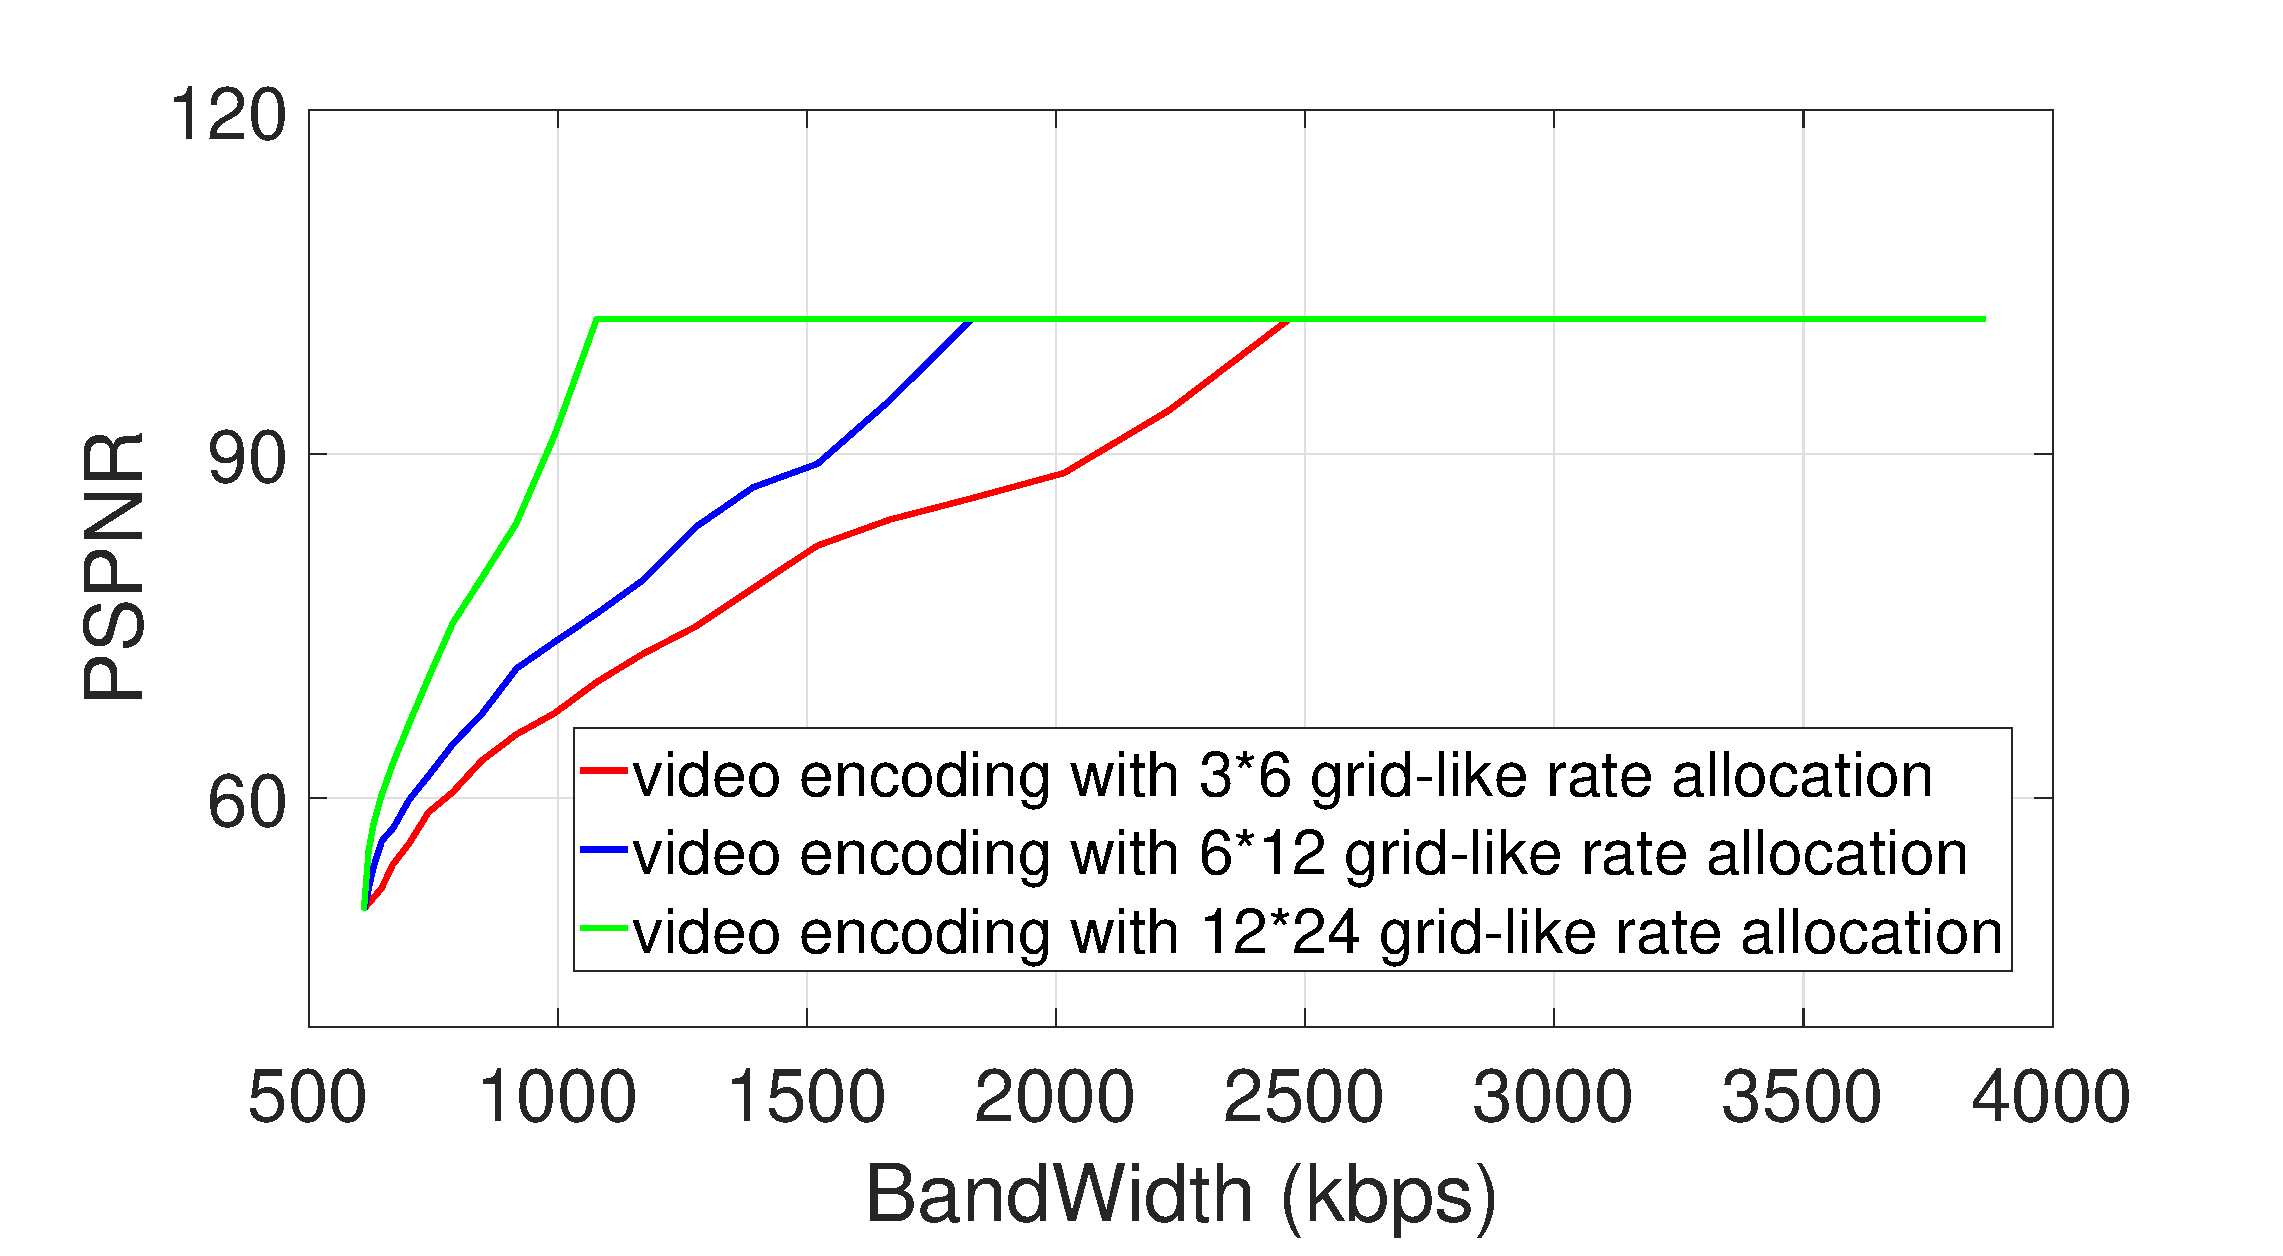
\includegraphics[width=2.5in]{images/optimalencoding.eps}
  \caption{PSPNR-bandwidth tradeoff in video encoding with different granularity of rate allocation.}
  \label{optimalencoding}
  \end{figure}

(2) Fine-grained tiling introduces serious bitrate efficiency problem in video encoding. In practice, each tile has to be encoded independently instead of encoded together. When we cut the video into tiles, the total video size is increased. Fig. \ref{bitrateefficiency} shows the video size of different tiling granularity compared with original video size. We find that cutting a video into 12*24 tiles introduces 50\% to 330\% additional video size compared to original video. This significantly lower its practical performance in perceived quality optimization, especially in low bandwidth situations where the bitrate efficiency problem is very serious.

\begin{figure}
  \centering
  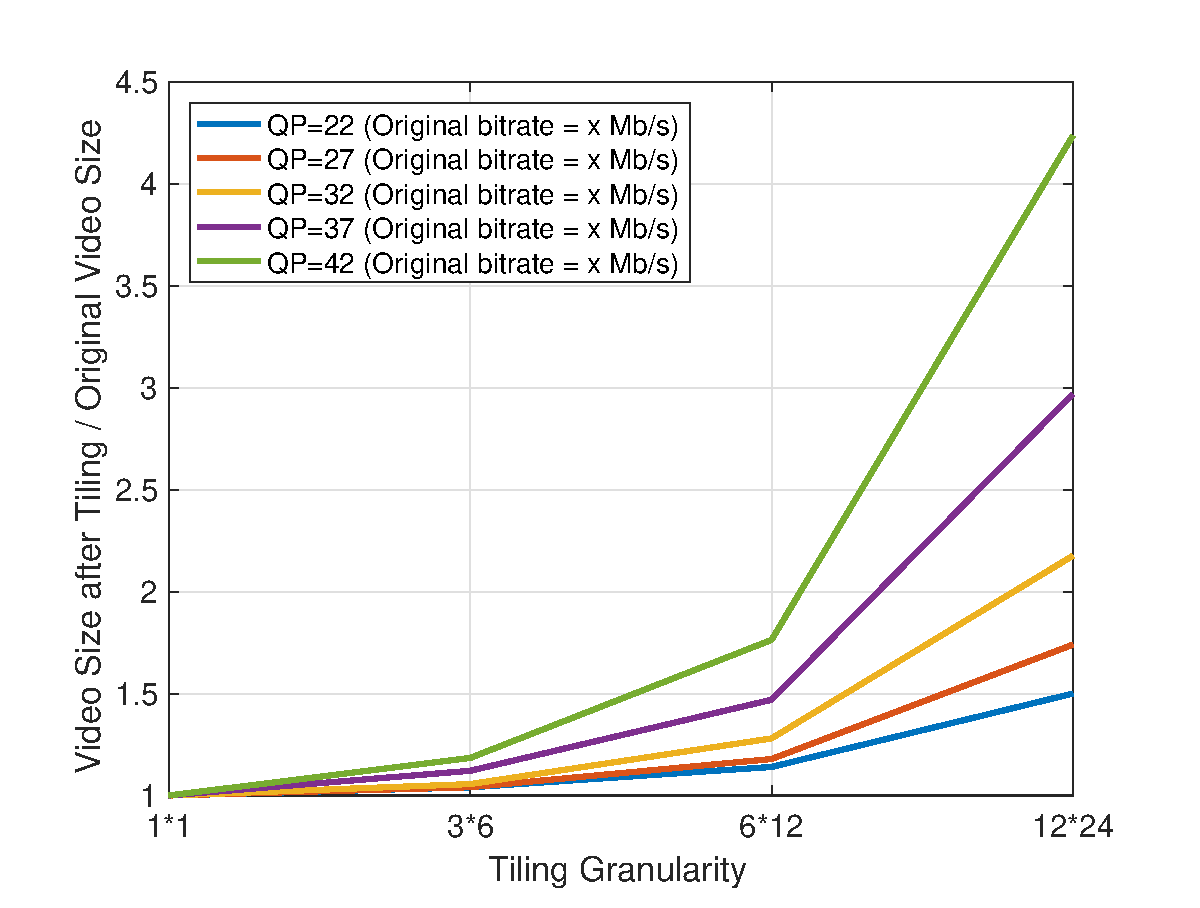
\includegraphics[width=2.5in]{images/bitrateefficiency.eps}
  \caption{The ratio of video size after tiling and original video size in each tiling granularity and each bitrate level. We notice that fine-grained tiling introduces serious bitrate efficiency problem, especially in low bandwidth situations in which the overall bitrate of each tile is low.}
  \label{bitrateefficiency}
  \end{figure}

\textbf{Challenge 3: Information needed for perceived quality computation is disparted on server-side and client-side.} 

To optimize perceived quality, client needs to compute the perceived quality of each bitrate allocation and then make decision. However, different from video quality which only related to video content itself, perceived quality depends on both video content and user behavior. Information of video content is located on server-side while information of user behavior is located on client-side. To get information of video content with current DASH, client has to pre-request in information of each pixel from server. This communication overload even exceed the overload of actual video streaming.

\subsection{Potential improvement}

As we have stated that perceived quality is not only related to object-viewpoint distance, it is also related to many factors, we need to clarify how much potential improvement can we get by taking above insights.

We set up a trace-driven experiment to evaluate this potential improvement. PSPNR \cite{PSPNR} is applied as a metric to measure perceived quality. Real traces are collected from over 800 VR displays of 48 users. In our experiment, each video has 5 different bitrate level. We compare the performance of 3 methods:

\begin{itemize}

\item \emph{Viewpoint-driven VR streaming.} Video is cut into 6*12 spatial rectangular tiles. Tiles on user's viewpoint is allocated the high bitrate. For other tiles, bitrate is allocated linearly decreasing with its distance to user's viewpoint.

\item \emph{Perceived quality driven VR streaming.} Suppose we can freely allocate bitrate to each spatial part of video without video tiling. With consideration of user viewpoint, content luminance and texture complexity, we do adaptive streaming to maximize user-perceived quality.

\item \emph{Perceived quality driven VR streaming. (with 3 VR factors)} Suppose we can freely allocate bitrate to each spatial part of video without video tiling. Besides user viewpoint, content luminance and texture complexity, we also take consideration of viewpoint moving speed, content Depth-of-Field and light / dark adaptation, we do adaptive streaming to maximize user-perceived quality.

\end{itemize}

\begin{figure}
  \centering
  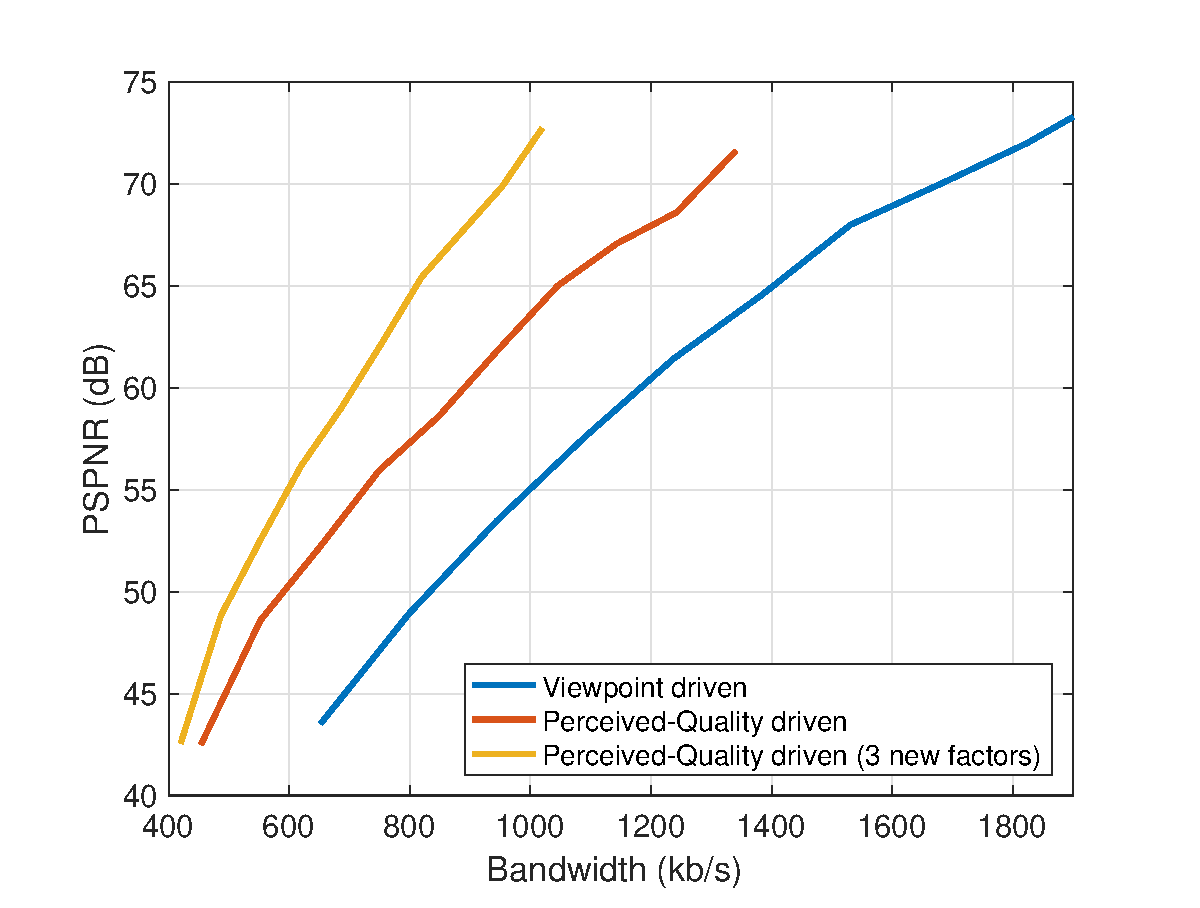
\includegraphics[width=2.5in]{images/improvement.eps}
  \caption{PSPNR-bandwidth tradeoff of (1) Viewpoint-driven VR streaming. (2) Perceived quality driven VR streaming. (3) Perceived quality driven VR streaming. (with 3 VR factors)}
  \label{potential1}
  \end{figure}

Fig. \ref{potential1} shows the PSPNR-bandwidth tradeoff of 3 strategies.

\textbf{Key observations:} 
\begin{itemize}
\item With consideration of content luminance and texture complexity, perceived-quality-driven VR streaming can save 30\% bandwidth compared with viewpoint-driven VR streaming providing the same PSPNR. Moreover, when we take consideration of viewpoint moving speed, object Depth-of-Field and light / dark adaptation, we can further save 20\% bandwidth.
\end{itemize}
\section{Key insights and ideas}

As stated in previous section, the biggest challenge of optimizing user-perceived quality is that perceived quality is related to both video content and user behavior. To solve the challenge, we show that perceived quality optimization can be decoupled: we can optimize video-content-related factors on server-side and optimize user-behavior-related factors on client-side.

\subsection{Insights}
In this section, we show that in VR streaming, each visual factor influences user-perceived quality independently. So we can decouple them into several single factors to measure perceived quality respectively, then we design an server-side offline tiling scheme only with consideration of video content, and design a client-side bitrate allocation method only with consideration of user behavior.

\textbf{Insight 1: Perceived quality model in VR display can be built by simply adding several new factors on traditional perceived quality model.}

In traditional video display, there are many factors which influence user-perceived quality. Prior works have studied how single factors influence user-perceived quality. Moreover, \cite{distance} proves that, in perceived quality computation, several factors (luminance, texture complexity, etc.) can be considered independently. As a result, we can independently measure the influence of each factor as a coefficient, and multiply them together to obtain the final user-perceived quality.

However, in VR display, there are some new factors which are never considered in traditional video display. So how these new factors, together with factors in traditional video display, influence the perceived quality in VR streaming, is an unknown problem. We intend to assume that they can also be computed independently, and then multiplied as coefficients together with traditional factors to obtain final user-perceived quality.

To prove our guess, we set up a user study to evaluate how perceived quality is influenced by multiple factors. (Sec. 4) Our result shows that perceived quality model in VR display can be decoupled. We only need to simply add new factors to traditional perceived quality model.

\textbf{Insight 2: Video tiling strategy can be optimized on server side.}

In traditional grid-like video tiling scheme, video is cut into m*n rectangular tiles with equal size. 

This tiling strategy has an obvious drawback: at most times the boundary between objects are not exactly on the boundary between two adjacent tiles. Fig. \ref{fig_insight_tiling} shows an example. In the video frame, there are two objects (Object A, Object B) and a background. In coarse-grained tiling (Fig. \ref{fig_insight_tiling}(b)), the object can not be exactly caught by one or several tiles. It leads to bitrate allocation of low performance. In fine-grained tiling (Fig. \ref{fig_insight_tiling}(c)), although the object can be caught by several tiles, it cut the video into too many tiles and many cutting lines are unnecessary. It leads to serious bandwidth efficiency problem as described in Sec. 2.3.

\begin{figure*}[!t]  
\begin{tabular}{cccc}  
\begin{minipage}[t]{0.24\linewidth}  
 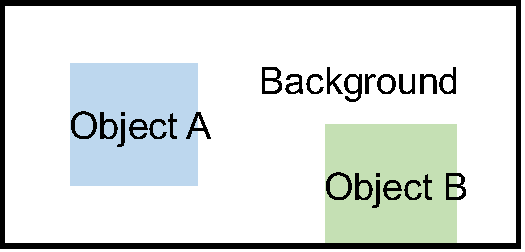
\includegraphics[width = 1\linewidth]{images/insight_tiling1.pdf}  
     \center{(a) A video frame.}
     \label{fig_insight_tilinga}
\end{minipage}  
\begin{minipage}[t]{0.24\linewidth}  
    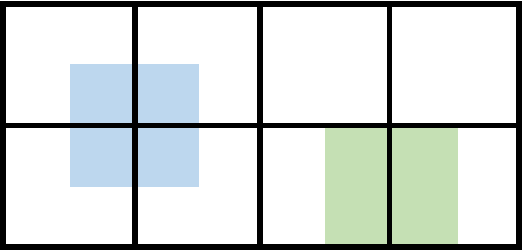
\includegraphics[width = 1\linewidth]{images/insight_tiling2.pdf}  
     \center{(b) Grid-like tiling in coarse granularity.}
     \label{fig_insight_tilingb}
\end{minipage}  
\begin{minipage}[t]{0.24\linewidth}  
 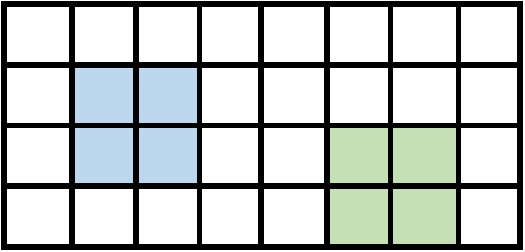
\includegraphics[width = 1\linewidth]{images/insight_tiling3.pdf}  
     \center{(c) Grid-like tiling in fine granularity.}
     \label{fig_insight_tilingc}
\end{minipage}  
\begin{minipage}[t]{0.24\linewidth}  
 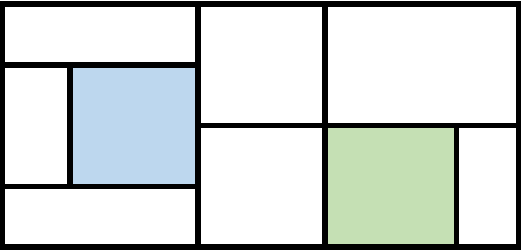
\includegraphics[width = 1\linewidth]{images/insight_tiling4.pdf}  
     \center{(d) Object-based tiling.}
     \label{fig_insight_tilingd}
\end{minipage}  
\end{tabular}  
  \caption{An example of traditional grid-like tiling and object-based tiling.}  
\label{fig_insight_tiling}
\end{figure*}  

Suppose we can know information about video content, we can cut the video based on objects like Fig. \ref{fig_insight_tiling}(d). In this method, we can obtain similar tiling granularity as Fig. \ref{fig_insight_tiling}(c) but remain similar tile numbers as Fig. \ref{fig_insight_tiling}(b). We think tiling scheme like Fig. \ref{fig_insight_tiling}(d) can outperform traditional grid-like tiling scheme. Moreover, since information of objects is only related to video content, it is totally independent from user. So object-based tiling can be completed offline on server-side.

\textbf{Insight 3: Perceived quality computation can be decoupled.}

Although accurately computing perceived quality needs the information of both video content and actual user behavior, we can precompute perceived quality of given video content with each possible user behavior situations on server-side, without any information of actual user behavior, and transform the computation result to client. Client only needs to choose the situation which match actual user behavior most, then uses given perceived quality value to approximate the actual perceived quality. Experimental results prove that we can obtain very good approximation accuracy with very little end-to-end exchanging overhead of computation result transforming. 

\subsection{Key ideas to solve the challenges}

Based on above insights, we decouple the visual characteristics due to video content and user viewpoint, and design a perceived quality driven VR streaming system which consider visual characteristics of video objects completely on server-side, and considers visual characteristics of user behavior completely on client-side. Specifically, we build our system based on following ideas:

\begin{itemize}

\item \emph{Measuring perceived quality in VR streaming by incrementally adding some new coefficients into traditional non-VR perceived quality model.} (\S 4)

\item \emph{Server-side offline video tiling only based on of video content.} (\S 5)

\item \emph{Server-side perceived quality precomputation and client-side approximation \& optimization.} (\S 6)

\end{itemize}

\section{Perceived quality measurement}

In this section we first introduce Peak Signal-to-Perceptible-Noise Ratio (PSPNR) \cite{PSPNR} which is used as metric for perceived quality measurement. Then, since PSPNR computation needs the Just-Noticeable-Distortion (JND) \cite{JND} value of each pixel, we present our JND definition based on human visual system in VR display.

\subsection{Perceived quality measuring by Just-Noticeable Distortion (JND) model}

Since user-perceived quality is a subjective thing, how to measure it becomes a problem. For example, it is very hard for a user to say the perceived quality of video A is 2 times better than that of video B, or it is just 1.7 times better.

Peak Signal-to-Perceptible-Noise Ratio (PSPNR) \cite{PSPNR} is an widely-accepted metric to measure perceived quality. It is defined based on Just-Noticeable-Distortion (JND) theory \cite{JND}. Given the original video frame and a compressed video frame, user can notice their difference only if the difference between them is above a visibility threshold. When the different is under this threshold, it will not detected by user. This threshold is called Just-Noticeable-Distortion.

Based on JND theory, PSPNR is defined by accumulating error of each pixel which can be detected by user:

\begin{alignat}{2}\
\label{f1} PSPNR = 20 \times \log_{10}\frac{255}{\sqrt{PMSE}}
\end{alignat}
\begin{alignat}{2}\
PMSE=E\{ \left[ |p(x, y) - \hat{p}(x, y)| - JND(x, y)\right]^2 \times \Delta (x, y)\}
\end{alignat}
\begin{alignat}{2}\
\Delta (x, y) =\left\{
\begin{aligned}
1, & &|p(x, y) - \hat{p}(x, y)| > JND(x, y) \\
0, & &|p(x, y) - \hat{p}(x, y)| \le JND(x, y)
\end{aligned}
\right.
\end{alignat}

where $p(x, y)$ and $\hat{p}(x, y)$ are value of pixel $(x, y)$ in original video frame and compressed video frame. $JND(x, y)$ is the visibility threshold of pixel $(x, y)$.

Compared with PSNR (which is widely used in evaluating video / image quality), the core difference of PSPNR is introducing a term $JND(x, y)$ for each pixel $(x, y)$. So how to compute JND for each pixel $(x, y)$ is an important issue. We will present our JND computation in the following section.

\subsection{Building Just-Noticeable-Distortion Model for VR display}
The just-noticeable distortion (JND) provides cues for measuring the visibility of the Human Vision System (HVS). JND refers to the maximum distortion which cannot be perceived by human. It describes the perceptual redundancy of the picture by providing the visibility threshold. The JND model generally exploits the visibility of the minimally perceptible distortion.

JND has been well-studied in traditional video display since 1995. The most basic and solid research is about the relationship between content luminance and JND. \cite{luminance1}  and \cite{PSPNR} prove that content with moderate content luminance have low JND value, while content with very high or very low content luminance have high JND value. (Fig. \ref{JNDluminance})

\begin{figure}
  \centering
  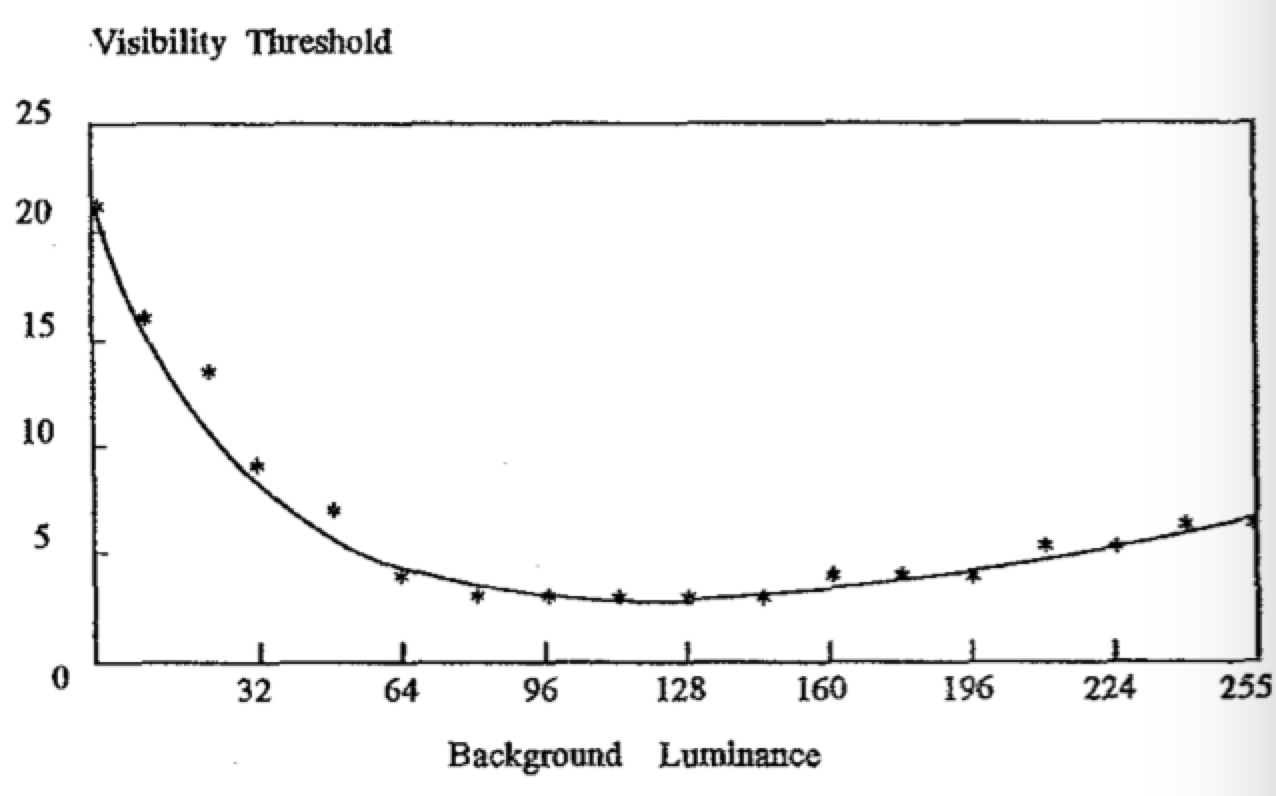
\includegraphics[width=2.5in]{images/backgroundluminance.jpg}
  \caption{JND due to content luminance.}
  \label{JNDluminance}
  \end{figure}

In recent years, based on the insight of content luminance - JND relationship, researchers have explored some more factors which are also related to JND, such as texture complexity, viewpoint-object distance (\cite{PSPNR}, \cite{distance}) and some other factors. Although the relationship between multiple JND factors may be complex, for simplicity, we can decouple them into several single factors. For example, \cite{distance} set up a user study to test the JND value with the combined effect of content luminance and viewpoint-object distance. The result proves that viewpoint-object distance can be considered independently from content luminance (Fig. \ref{JNDlum-dist}). It can be regarded as a coefficient which can be directly multiplied on JND value computed by content luminance. Based on this insight, JND computation for multiple factors is decoupled into several single factors. This significantly simplify the JND computation.

\begin{figure}
  \centering
  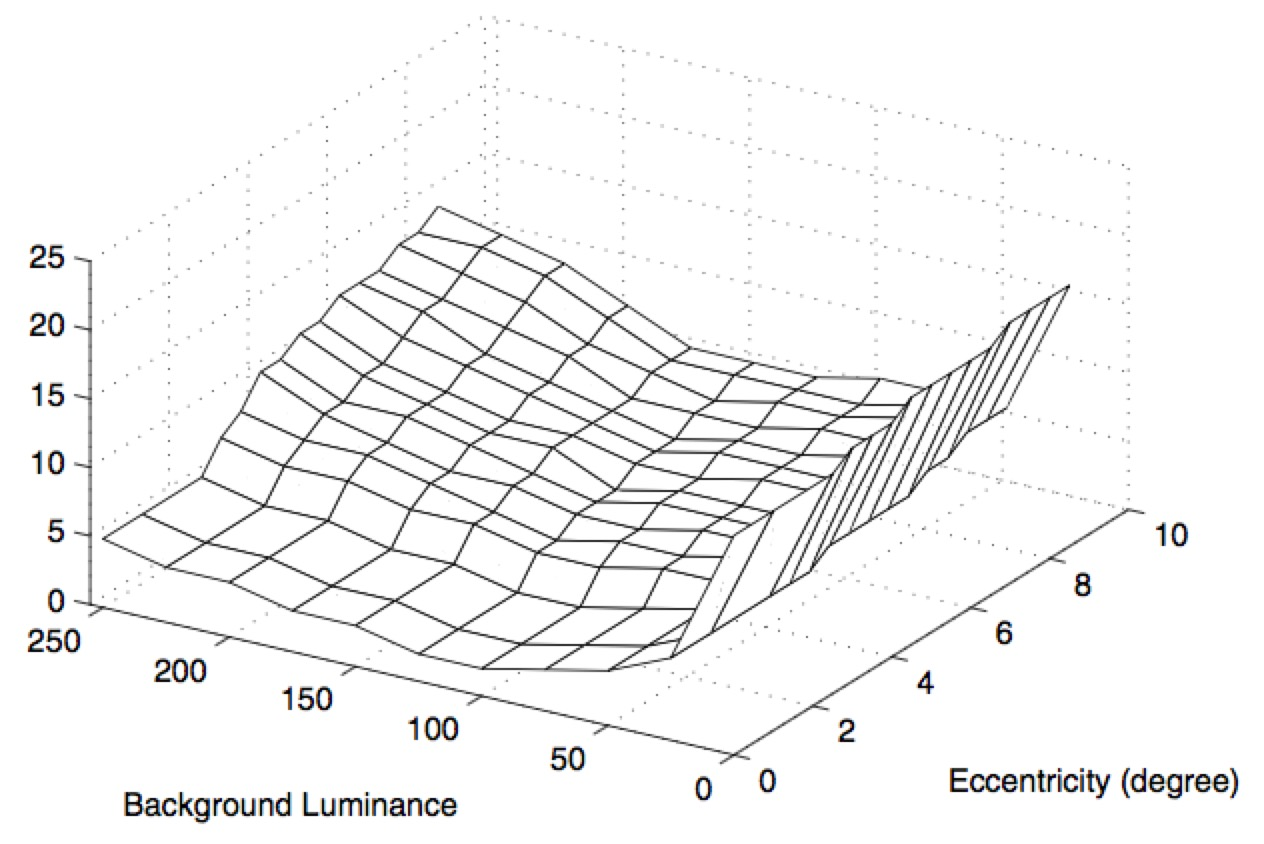
\includegraphics[width=2.5in]{images/JNDlum-dist.jpg}
  \caption{JND due to content luminance \& viewpoint-object distance.}
  \label{JNDlum-dist}
  \end{figure}

In VR display, user experience is very different because 3 new factors should be taken into consideration: (1) viewpoint moving decreases visual acuity, (2) low Depth-of-Field decreases visual acuity and (3) light / dark adaptation decreases visual acuity. So previous JND model for traditional video display can not be directly applied on VR video display. Moreover, it is unknown that (1) how these new factors influence JND with combined effect of old factors, and (2) if they can also be decoupled into several single factors, like viewpoint-object distance \cite{distance}.

Strictly answering these 2 questions needs to test JND value for each possible combinations of all factors (including all possible luminance, texture, viewpoint-object distance, viewpoint moving speed, Depth-of-Field and light / dark adaptation, which make up a 6-dimension feature space), which is not practical for a real-world user study. For simplicity, we imitate the user study in \cite{distance}, which makes only 2 factors variable and other 4 factors fixed, then we can know how is the combined effect of the 2 factors to JND, and if they can be decoupled to 2 single factors which independently influence JND.

So we present 3 user studies: (1) JND v.s. luminance \& viewpoint moving speed. (2) JND v.s. luminance \& depth of field. (3) JND v.s. luminance \& light / dark adaptation. We evaluate the effect of 3 VR-only factors to JND, each with combined effect of luminance, since luminance is the most well-studied JND factor.

We conduct the user study using real Head Mounted Device (HMD). Parameters of proposed HMD are listed as Table \ref{table1}:

\begin{table}[h]
\centering
\caption{HMD Parameters}\label{table1}
\begin{tabular}{|p{3.5cm}|p{3.5cm}|}
\hline
Equipment & Oculus GO\\
CPU & Xiaolong 821 customized drive Edition\\
Memory & 3GB\\
Screen Resolution & 2560 $\times$ 1440\\
Refresh Rate & 72Hz\\
Fixed pupil distance & 63.5mm\\
\hline
\end{tabular}
\end{table}

X subjects participated in the experiments, including X males and X females. All of them were in their twenties. The subjects obtained extensive practice during the experiments.

In this paper, we imitate the human visibility experiments in \cite{PSPNR}. In the experiment, a small square area, 32 x 32 pixels, is located in the center of a flat field of constant grey level (luminance). For each possible grey level (luminance) of the square area, the noises of fixed amplitude are randomly added to or subtracted from the pixels within the square area. Through varying the amplitude of the noise, the visibility threshold for each grey level is determined when the square region contaminated by the noises is just noticeable. 

Experimental settings of our 3 user studies are:

1. \textbf{JND v.s. luminance \& viewpoint moving speed} Set a background with constant grey level and set the 32 * 32 square with 5 different grey levels: 30, 80, 130, 180 and 230. The square is doing uniform rectilinear motion on the background. Noises are randomly added to or subtracted from it. We test the visibility threshold in 2 conditions: (1) Observer's viewpoint is gazed on a fixed point and the square moves across the fixed point. (set the moving speed of 32*32 square area to 2 deg /s, 4 deg / s, 6 deg / s, 8 deg / s, 10 deg / s) (2) Observer's viewpoint is allowed to tracking the moving object. (set the moving speed of 32*32 square area to 5 deg /s, 10 deg / s, 20 deg / s, 40 deg / s, 80 deg / s)

2. \textbf{JND v.s. luminance \& depth of field} Set a background with constant grey level and set the 32 * 32 square with 5 different grey levels: 30, 80, 130, 180 and 230. Then set the depth-of-field of the square to 2m, 10m, 50m. Testing the visibility threshold for these situations.

3. \textbf{JND v.s. luminance \& light / dark adaptation} Before our test, we show subjects a pure background with gray level $L_A$ ($L_A$ = 30, 80, 130, 180, 230) for 20 seconds. Then we change the background gray level to $L_B$ ($L_B$ = 30, 80, 130, 180, 230) and show subjects the 32*32 square. Testing the visibility threshold for these situations.

\subsection{Results}

\subsubsection{JND v.s. luminance \& viewpoint moving speed}

One of the most highlighted feature of VR video is that users can freely move their viewpoints. According to our data analysis, more than 30\% viewpoints are moving faster than 20 deg/s. (Fig. \ref{CDFspeed}) When human viewpoint is moving, visual acuity is decreased in 2 different conditions: (1) if user is tracking an object, visual acuity decreases smoothly with viewpoint moving speed increases. (2) If user is not tracking an object, visual acuity decreases dramatically with viewpoint moving speed increases. \cite{speed}

\begin{figure}
  \centering
  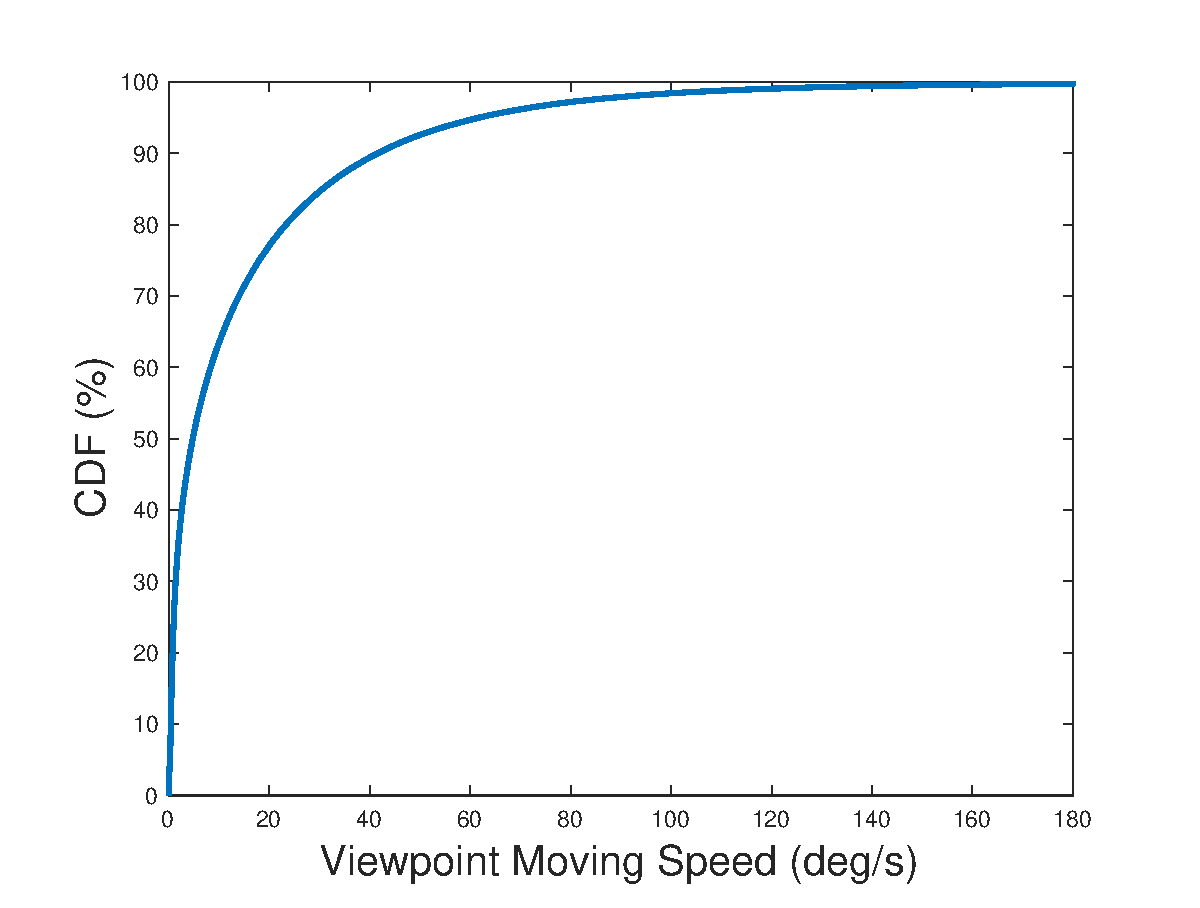
\includegraphics[width=2.5in]{images/speed_CDF.eps}
  \caption{CDF gram of viewpoint moving speed.}
  \label{CDFspeed}
  \end{figure}
  
We first analyze tracking condition. Fig. \ref{JNDspeed-lum-track} shows $JND_{lum\&speed}^{track}(l, v)$, the combined effect of viewpoint moving speed $v$ and content luminance $l$ to JND. We notice that effect of $v$ to $JND_{lum\&speed}^{track}$ is very similar in different $l$, so this combined effect can be decoupled into 2 parts:

\begin{figure}
  \centering
  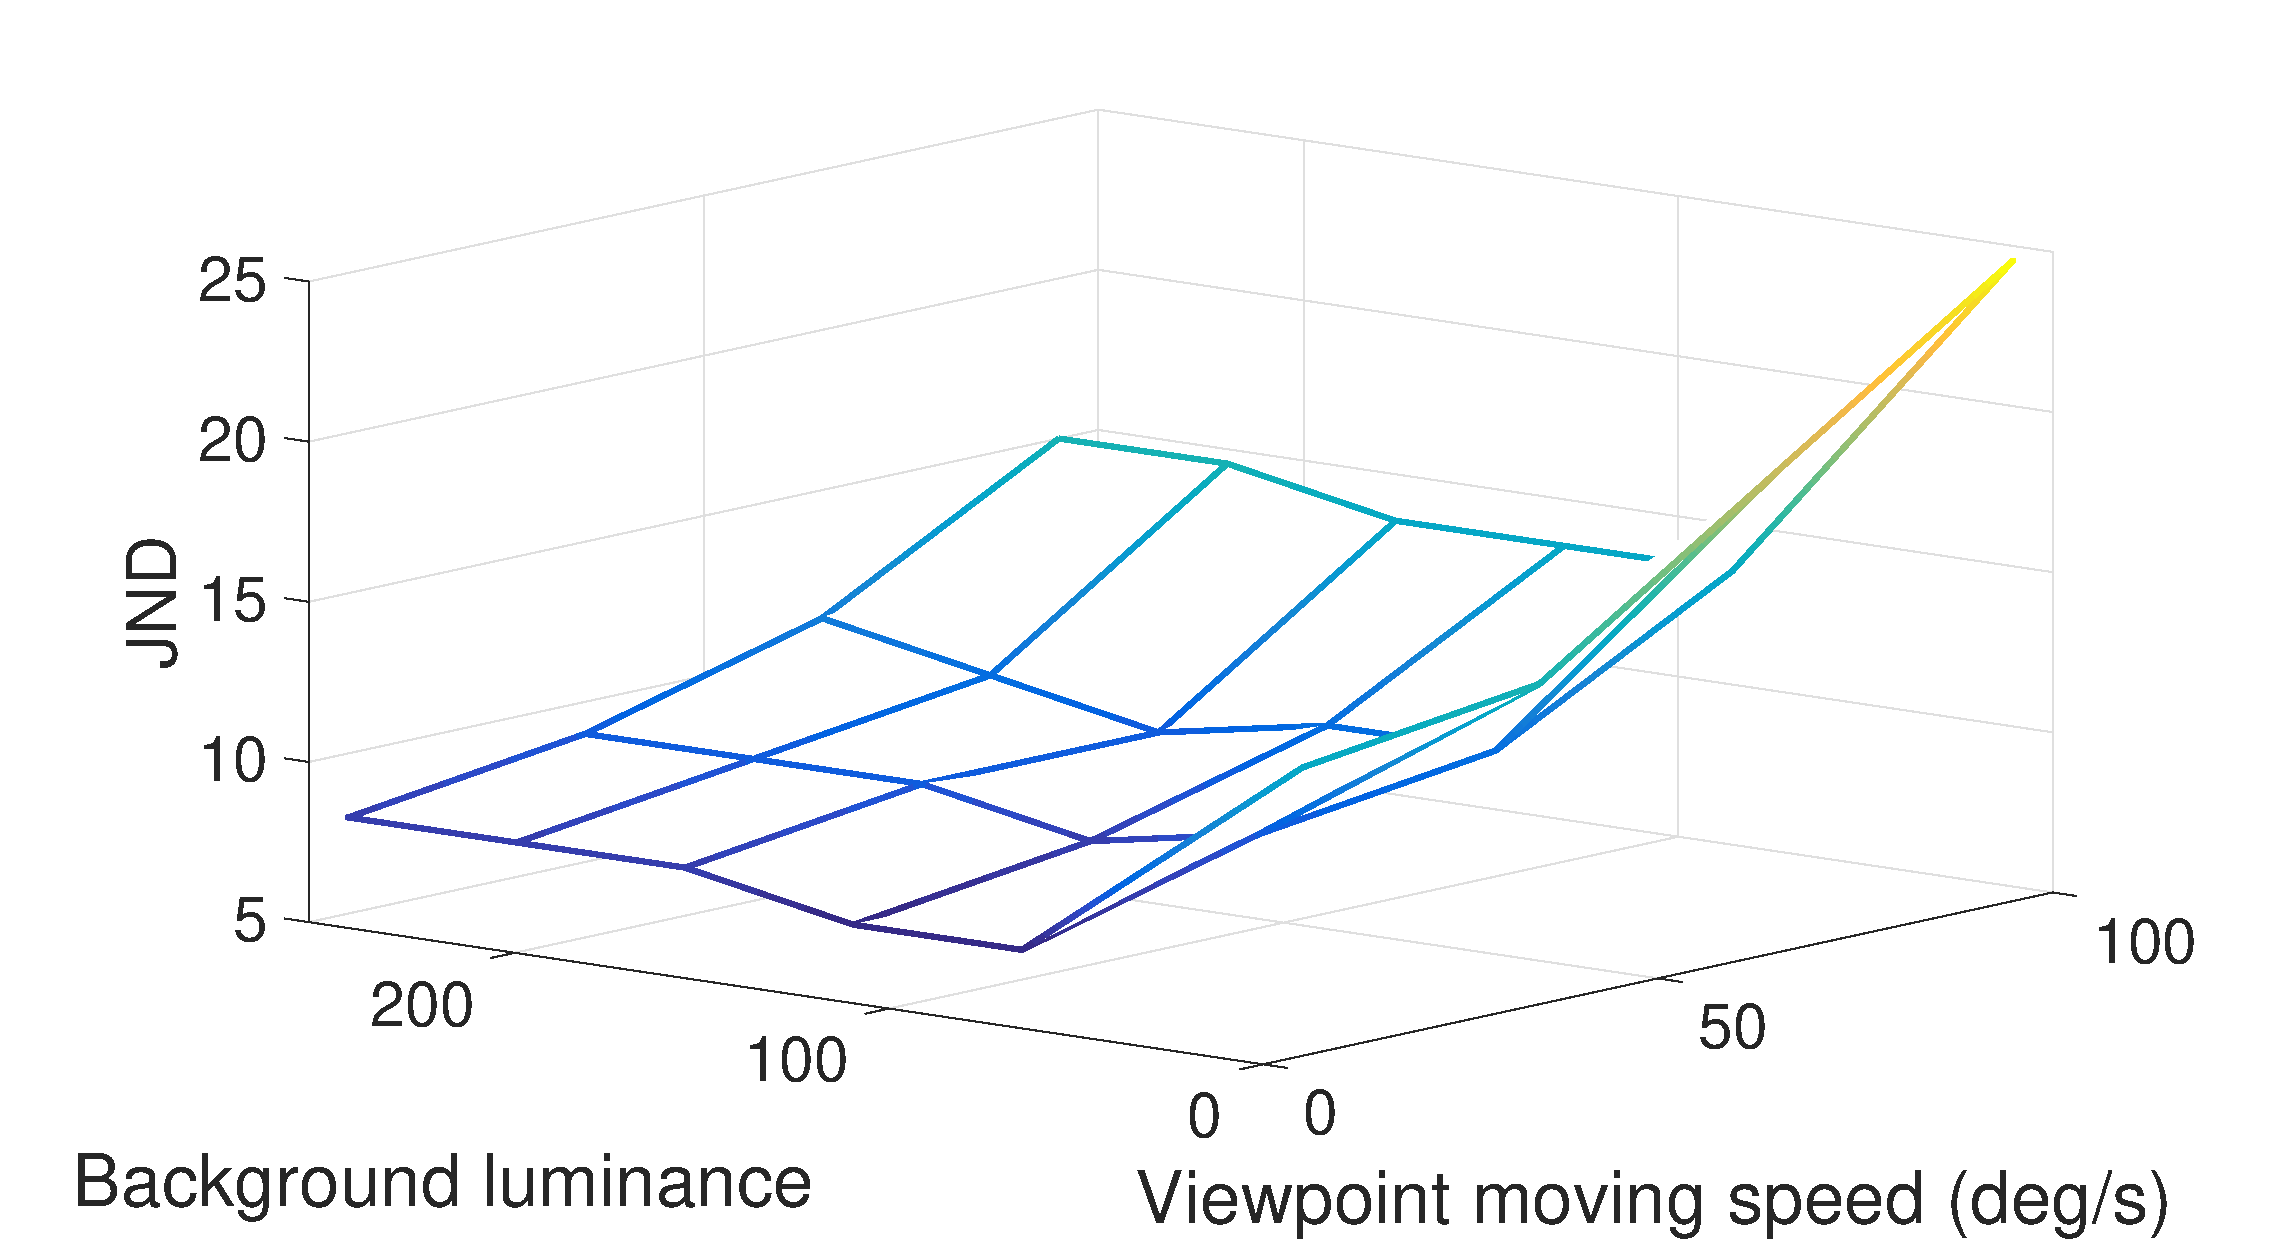
\includegraphics[width=2.5in]{images/JNDspeed-lum.eps}
  \caption{JND due to content luminance and viewpoint moving speed.}
  \label{JNDspeed-lum-track}
  \end{figure}

\begin{alignat}{2}\
JND_{lum\&speed}^{track}(l, v) = f_{lum}(l) \times f_{track}(v)
\end{alignat}

where $f_{lum}(l)$ represents the visibility threshold with only consideration of content luminance, and $f_{track}(v)$ is a coefficient which represents influence of viewpoint moving speed on visibility threshold.

$f_{lum}(l)$ has been presented as Fig. \ref{JNDluminance}. According to curve fitting, we can obtain $f_{track}(v) = \frac{JND_{lum\&speed}^{track}(l, v)}{f_{lum}(l)}$ as Fig. \ref{JNDspeed-track}.

\begin{figure}
  \centering
  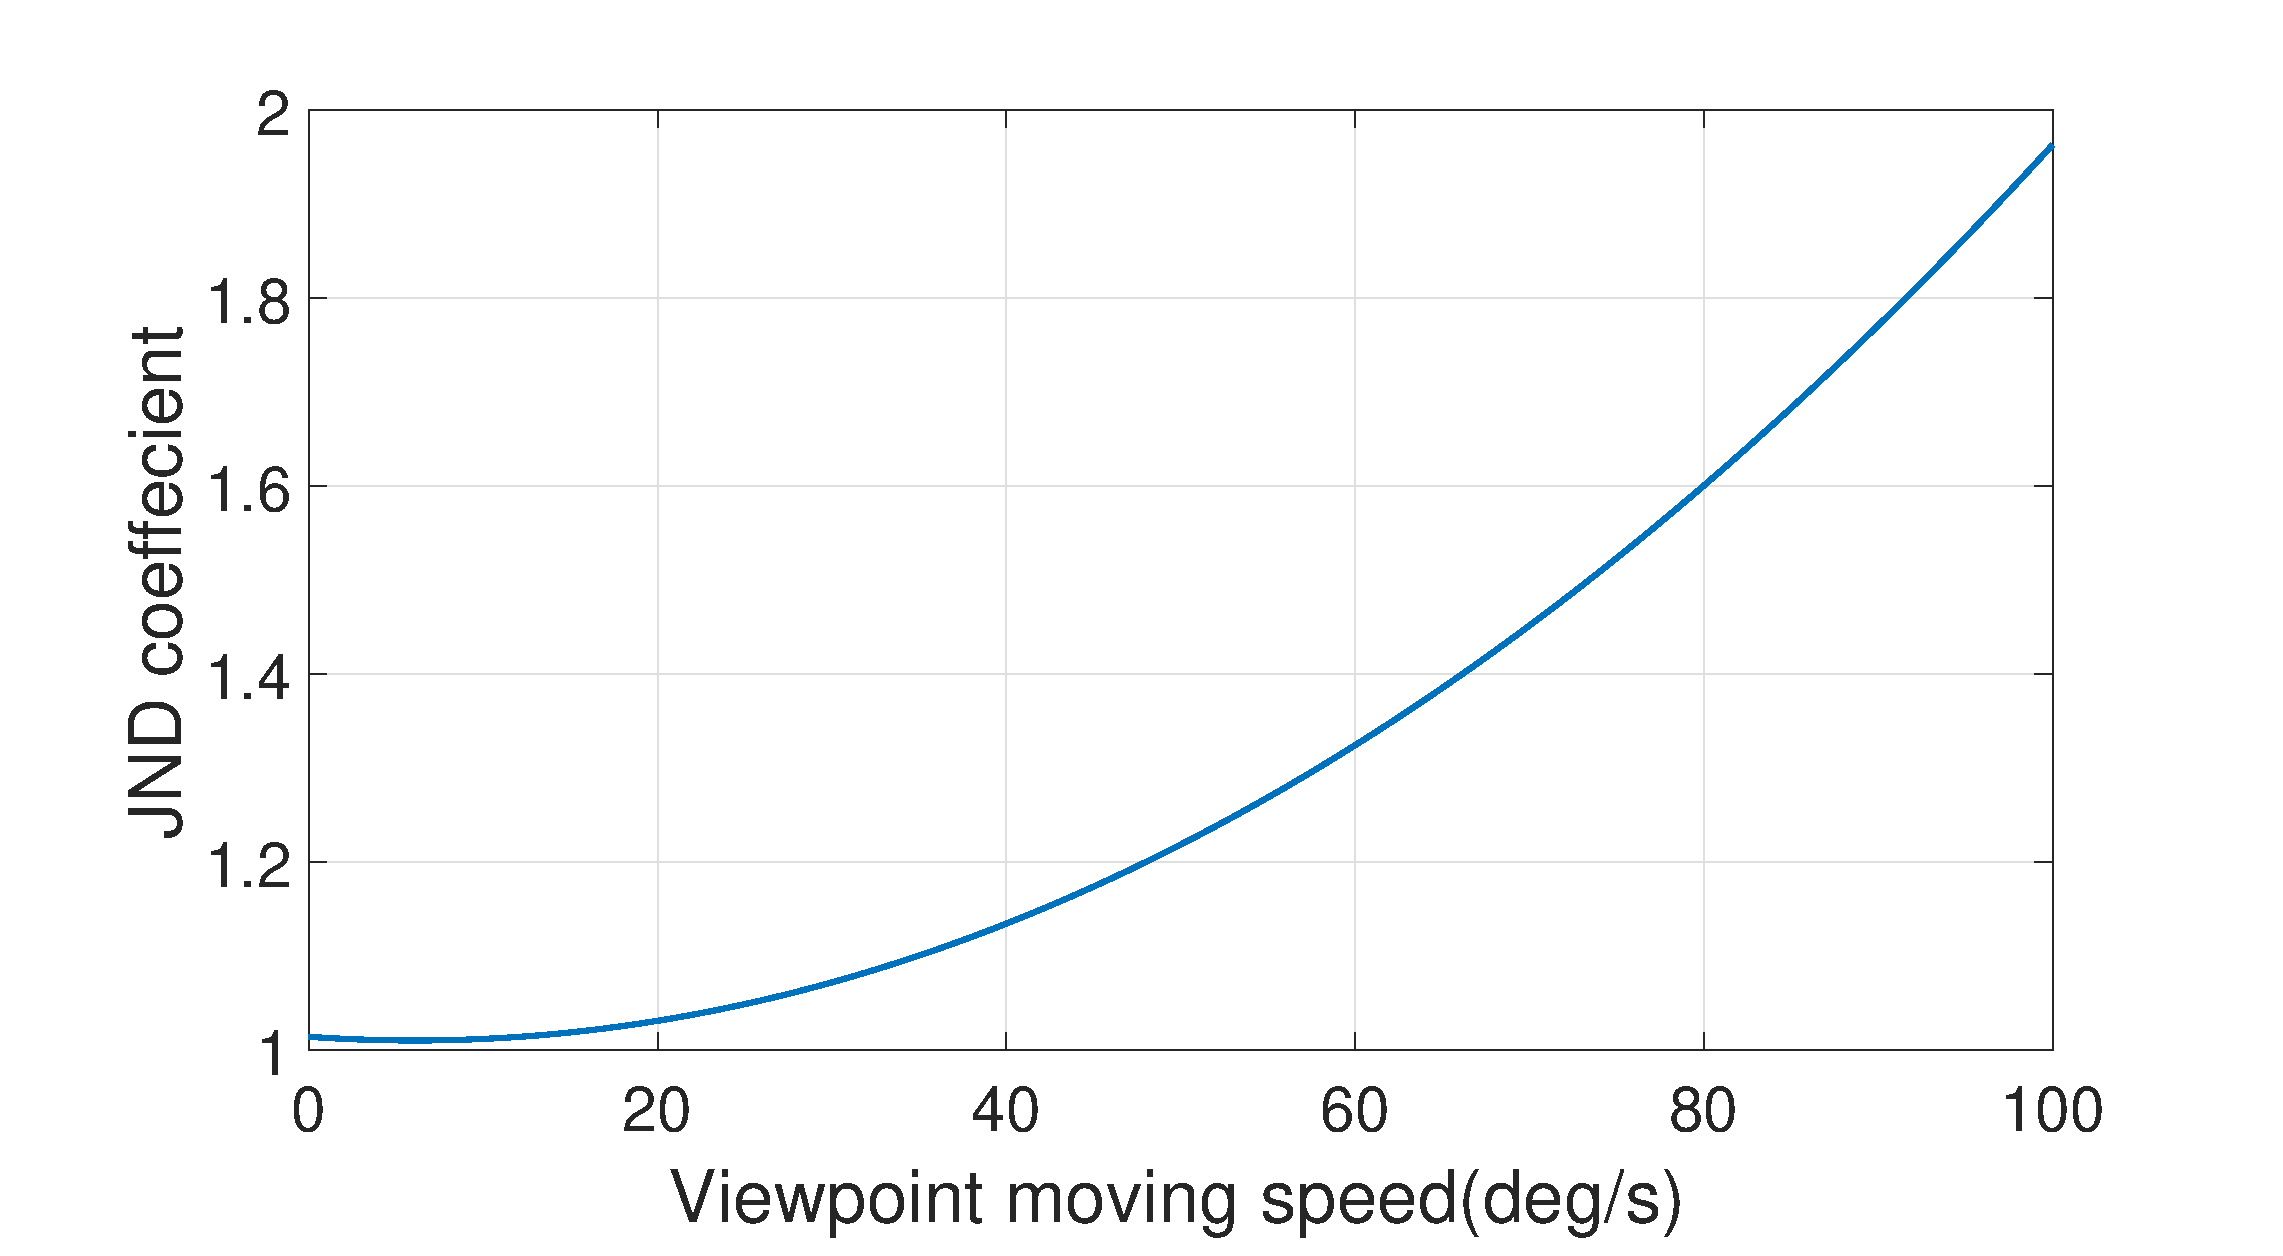
\includegraphics[width=2.5in]{images/JNDspeed.eps}
  \caption{$f_{track}(v)$, the JND coefficient of viewpoint moving speed.}
  \label{JNDspeed-track}
  \end{figure}

With similar method, we obtain result of no-tracking condition, $f_{notrack}(v)$, as Fig. \ref{JNDspeed-notrack}.

\begin{figure}
  \centering
  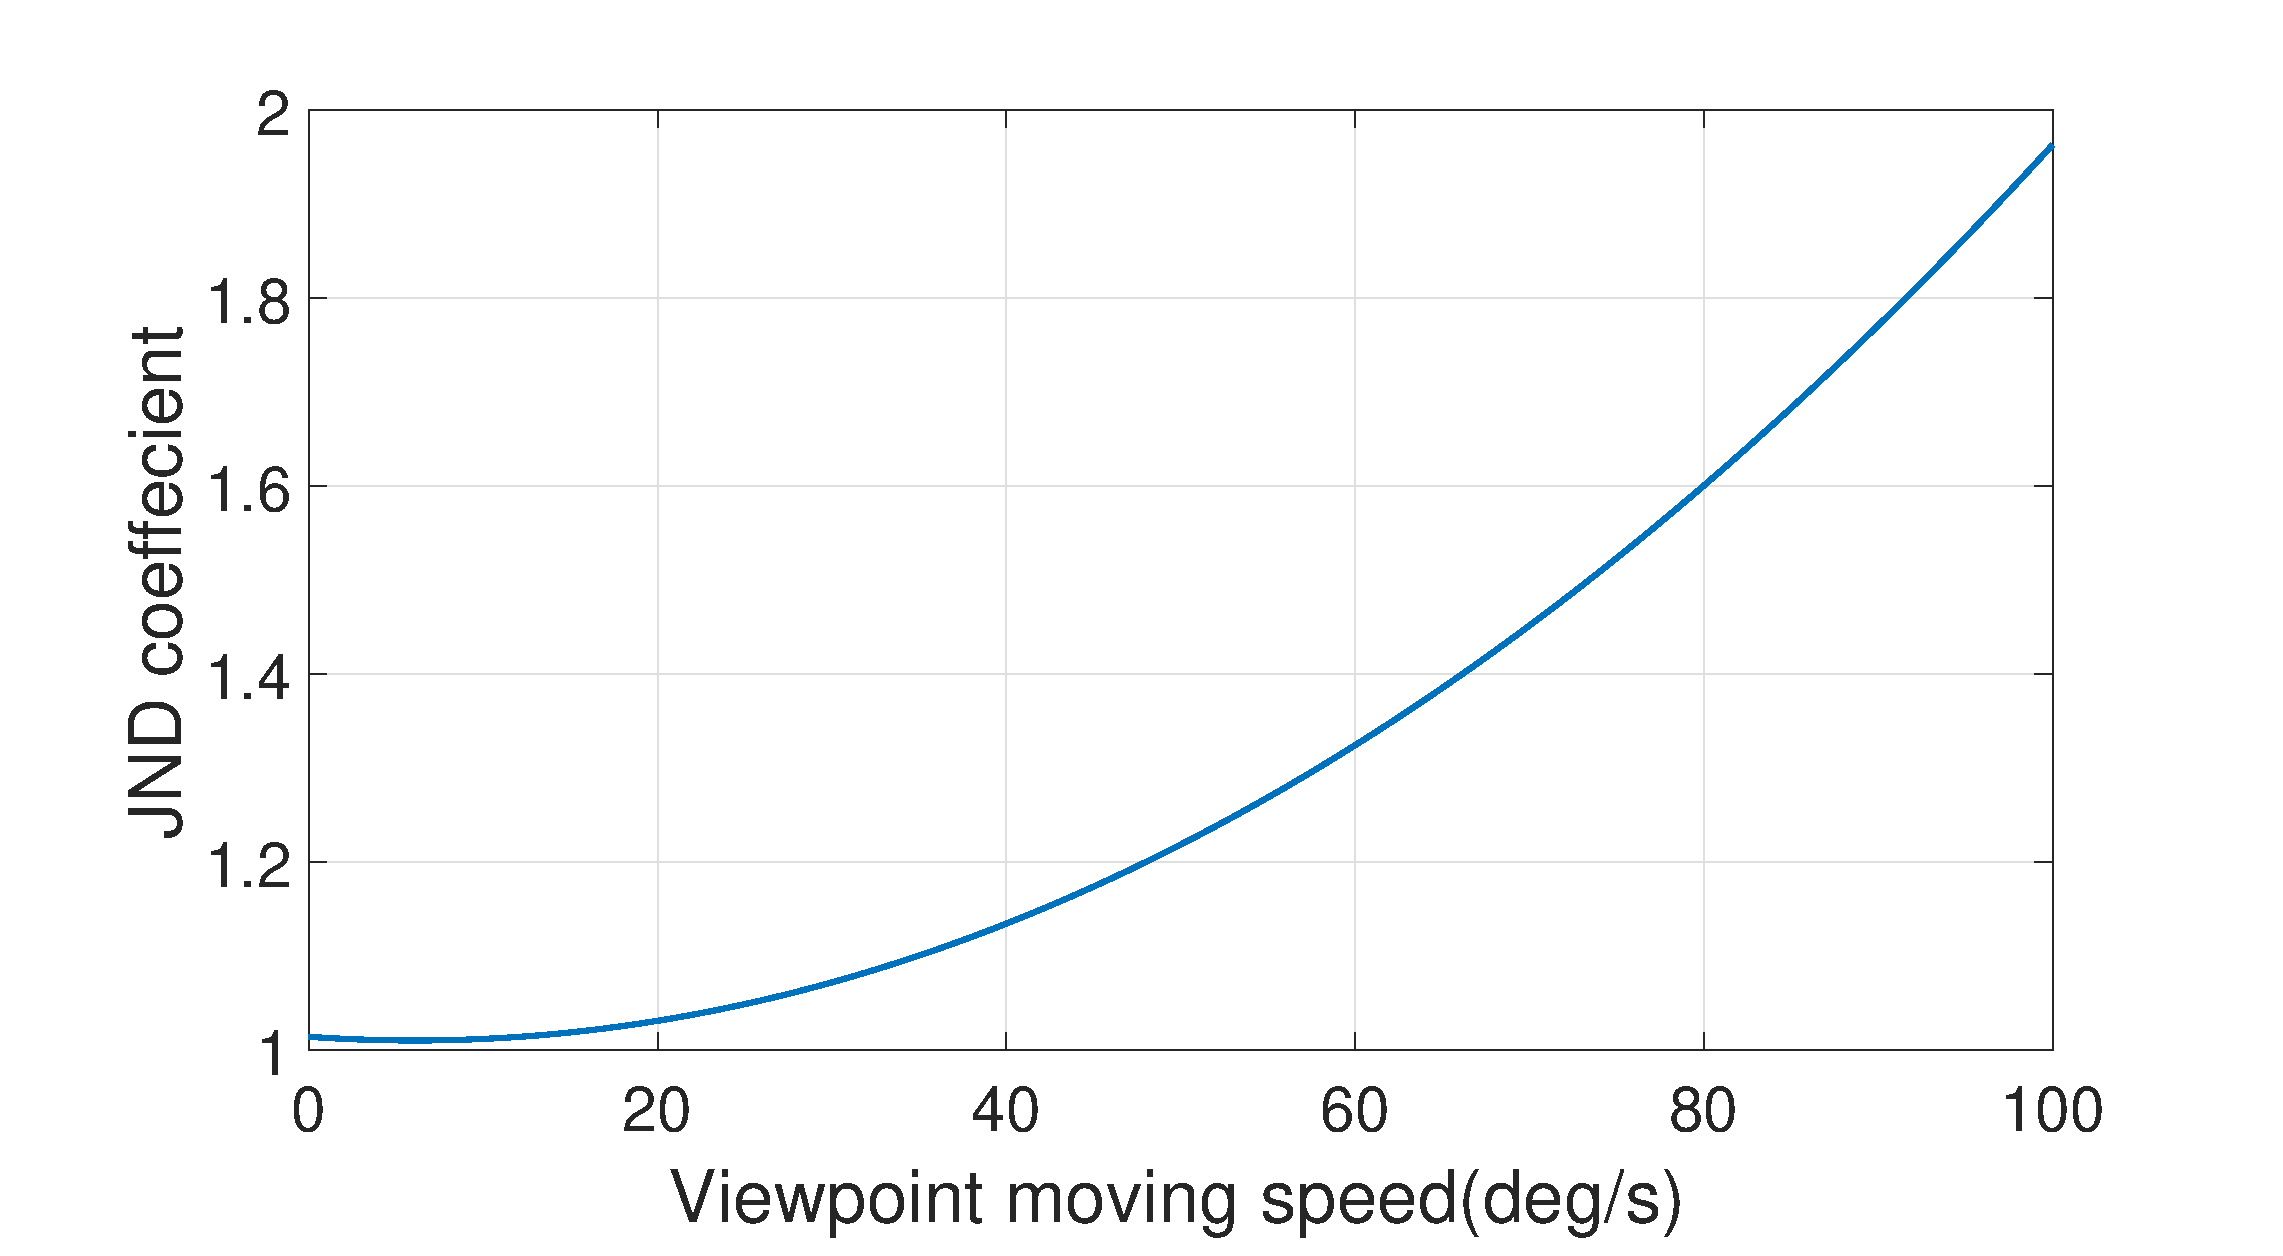
\includegraphics[width=2.5in]{images/JNDspeed.eps}
  \caption{$f_{notrack}(v)$, the JND coefficient of viewpoint moving speed.}
  \label{JNDspeed-notrack}
  \end{figure}

\subsubsection{JND v.s. luminance \& depth of field}

Depth-of-field (DoF) refers to the 3D distance from the object to human eyes. In real world, human detect object's DoF by parallax effect (Fig. \ref{v-aconflict}). When a human is looking at an object, the object's location is different in his left eye and right eye. When the object is only 10cm to human eyes, its location in 2 eyes are significantly different. When the object is 100m from human eyes, its location in 2 eyes are almost the same. Then human brain combines 2 different 2D images from 2 eyes and build a 3D image with Depth-of-Field. Plenty of works [] state that when human brain received 2 highly different image from left and right eye, combining them is hard and slow. So visual acuity decreases when human is looking at an object with small DoF.

\begin{figure}
  \centering
  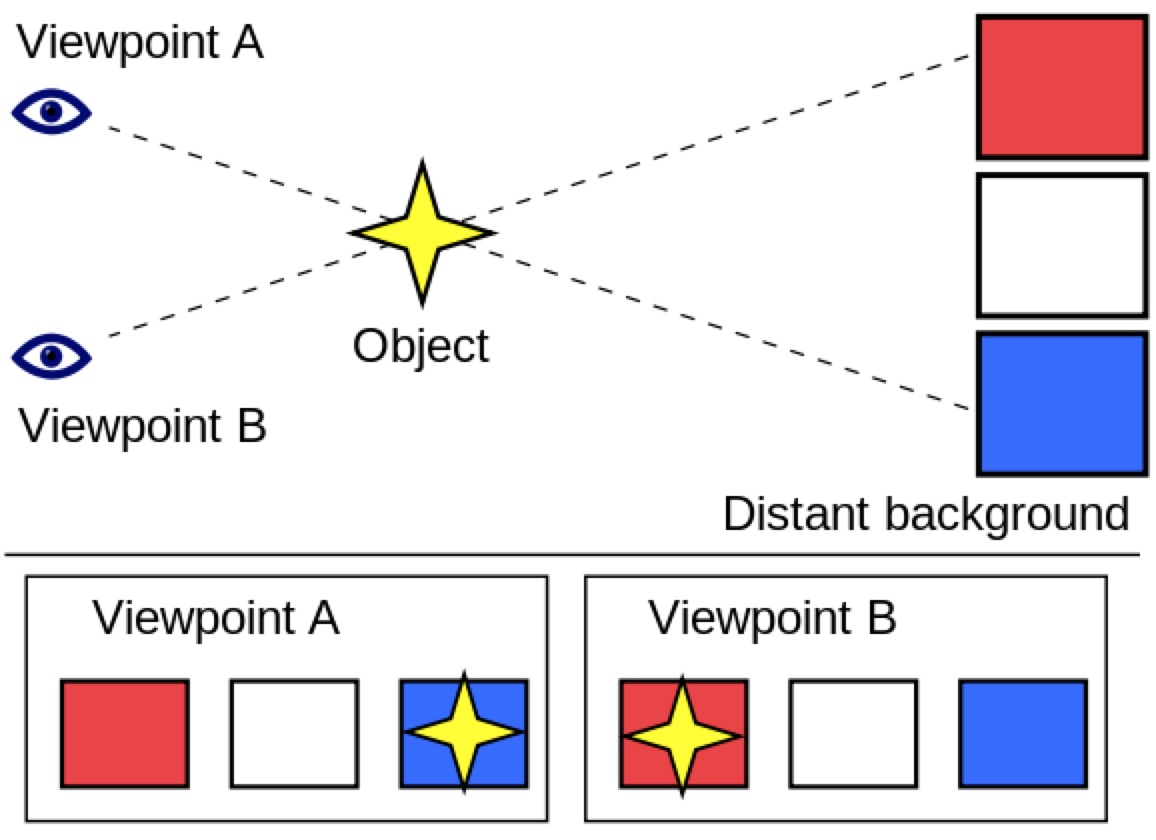
\includegraphics[width=2.5in]{images/ver-acc.jpg}
  \caption{An example of parallax effect.}
  \label{v-aconflict}
  \end{figure}

In non-VR video displays, the screen is bioptic, where only a single display is presented that is viewed by both eyes, so contents have the same DoF (in this situation the DoF is exactly the distance from eyes to screen) However, in most VR video displays, the screen is stereoscopic, where the illusion of depth is created by delivering images rendered from different angles to each eye. So left eye and right eye receives different image. As a result, in VR display, contents have different DoF.

Fig. \ref{JNDdof-lum} shows $JND(l, D)$, the combined effect of DoF $D$ and content luminance $l$ to JND. We notice that influence of DoF to JND is very similar in different content luminance, so this combined effect can be decoupled into 2 parts:

\begin{figure}
  \centering
  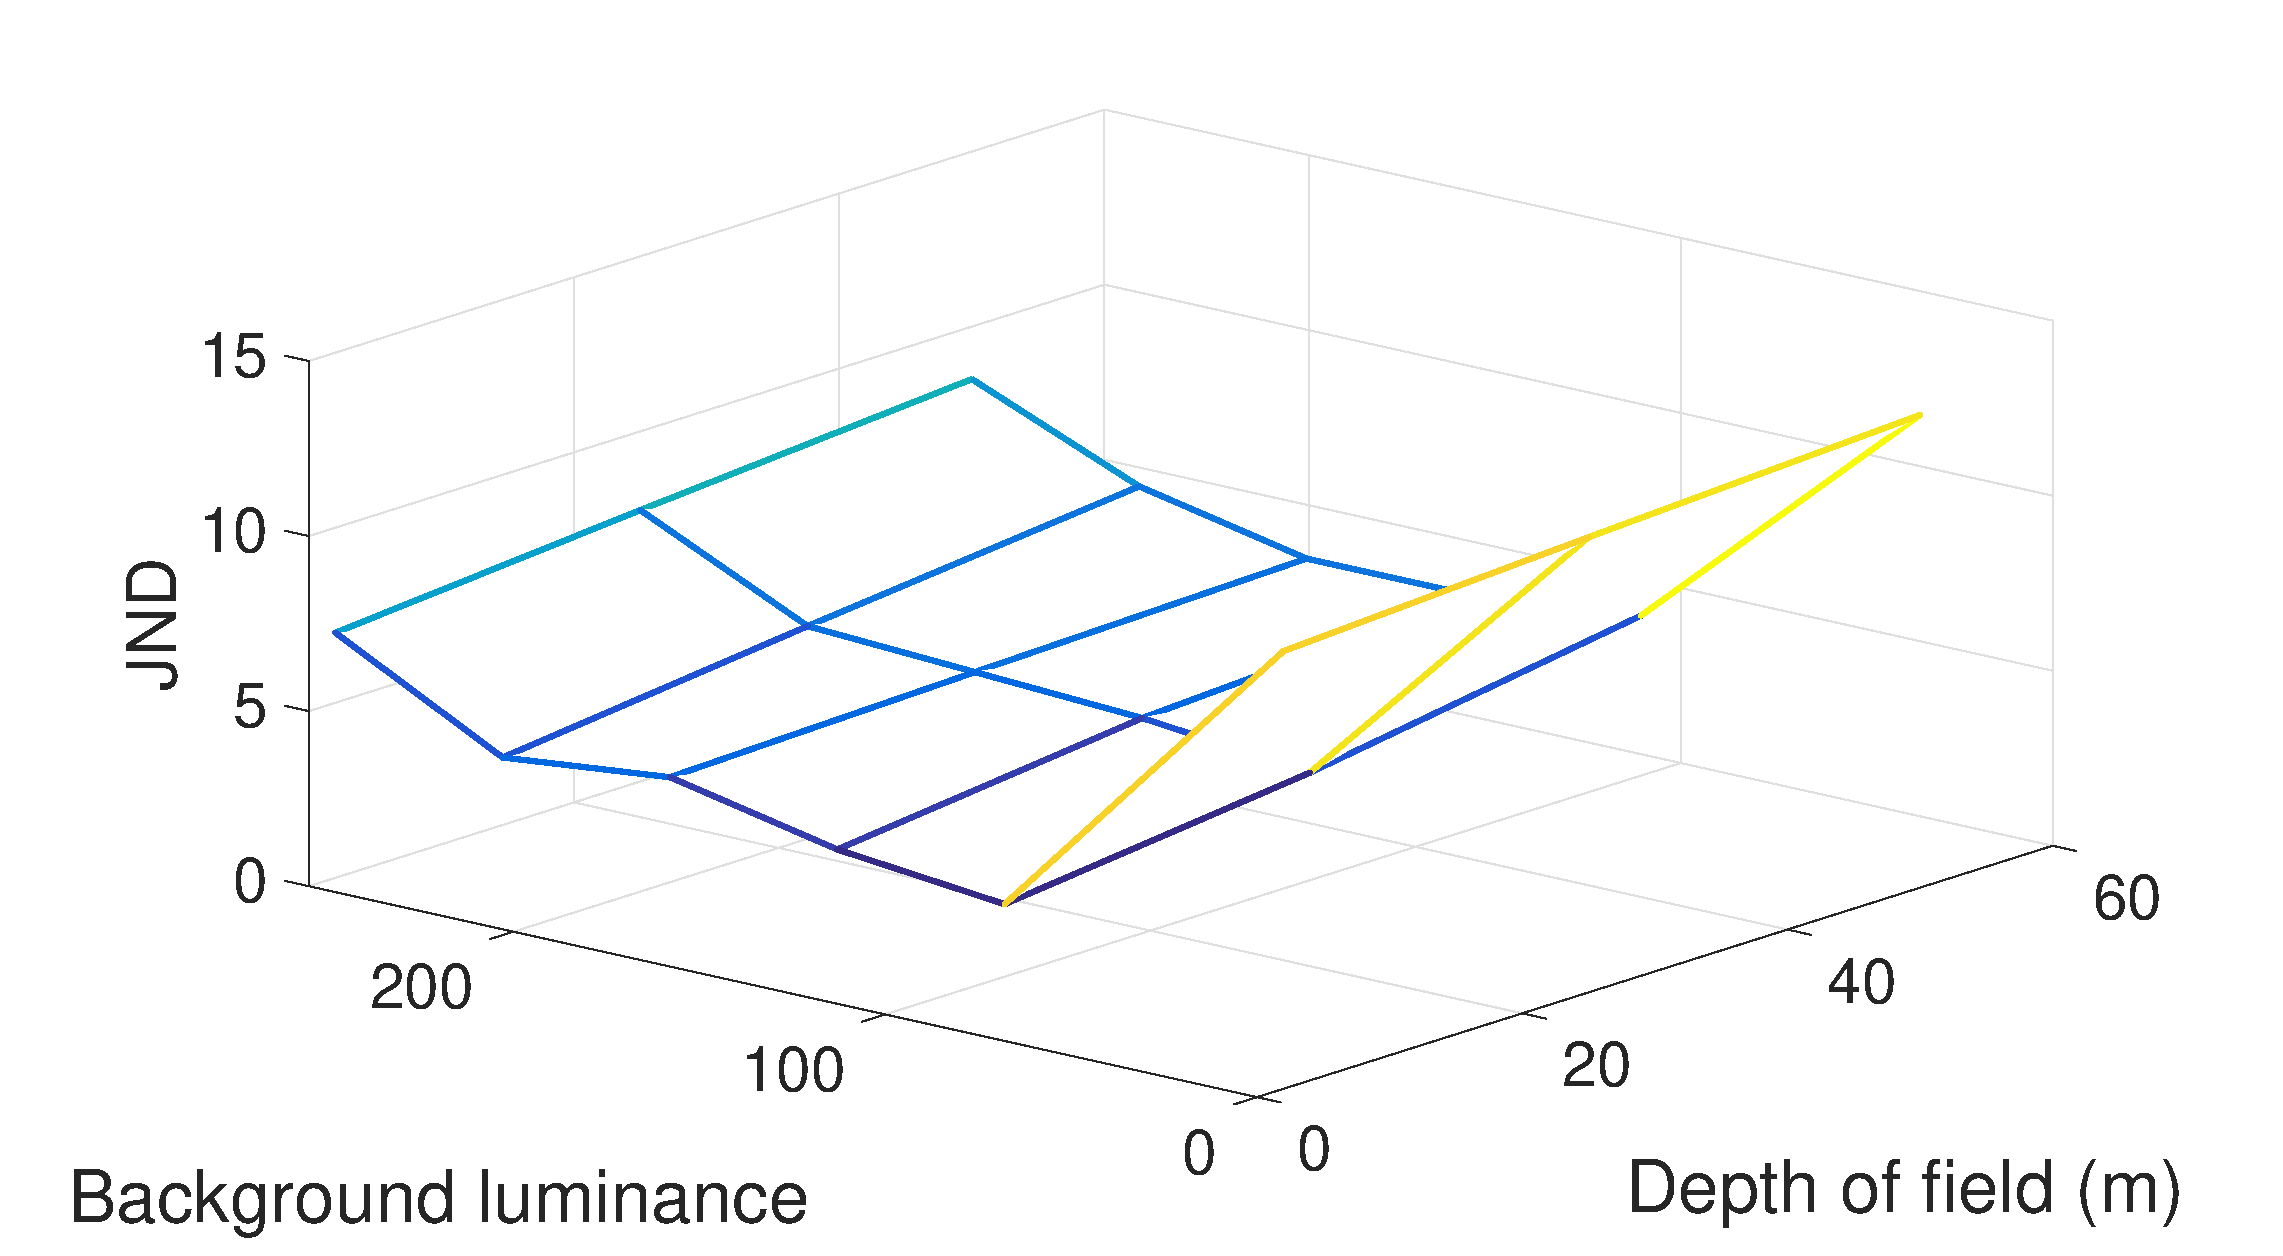
\includegraphics[width=2.5in]{images/JNDdof-lum.eps}
  \caption{JND due to content luminance and Depth-of-Field.}
  \label{JNDdof-lum}
  \end{figure}

\begin{alignat}{2}\
JND_{lum\&DoF}(l, D) = f_{lum}(l) \times f_{DoF}(D)
\end{alignat}

where $f(_{lum}(l))$ represents the visibility threshold with only consideration of content luminance, and $f_{DoF}(D)$ is a coefficient which represents DoF's influence on visibility threshold.

$f_{lum}(l)$ has been presented as Fig. \ref{JNDluminance}. According to curve fitting, we can obtain $f_{DoF}(D) = \frac{JND_{lum\&DoF}(l, D)}{f_{lum}(l)}$ as Fig. \ref{JNDdof}.

\begin{figure}
  \centering
  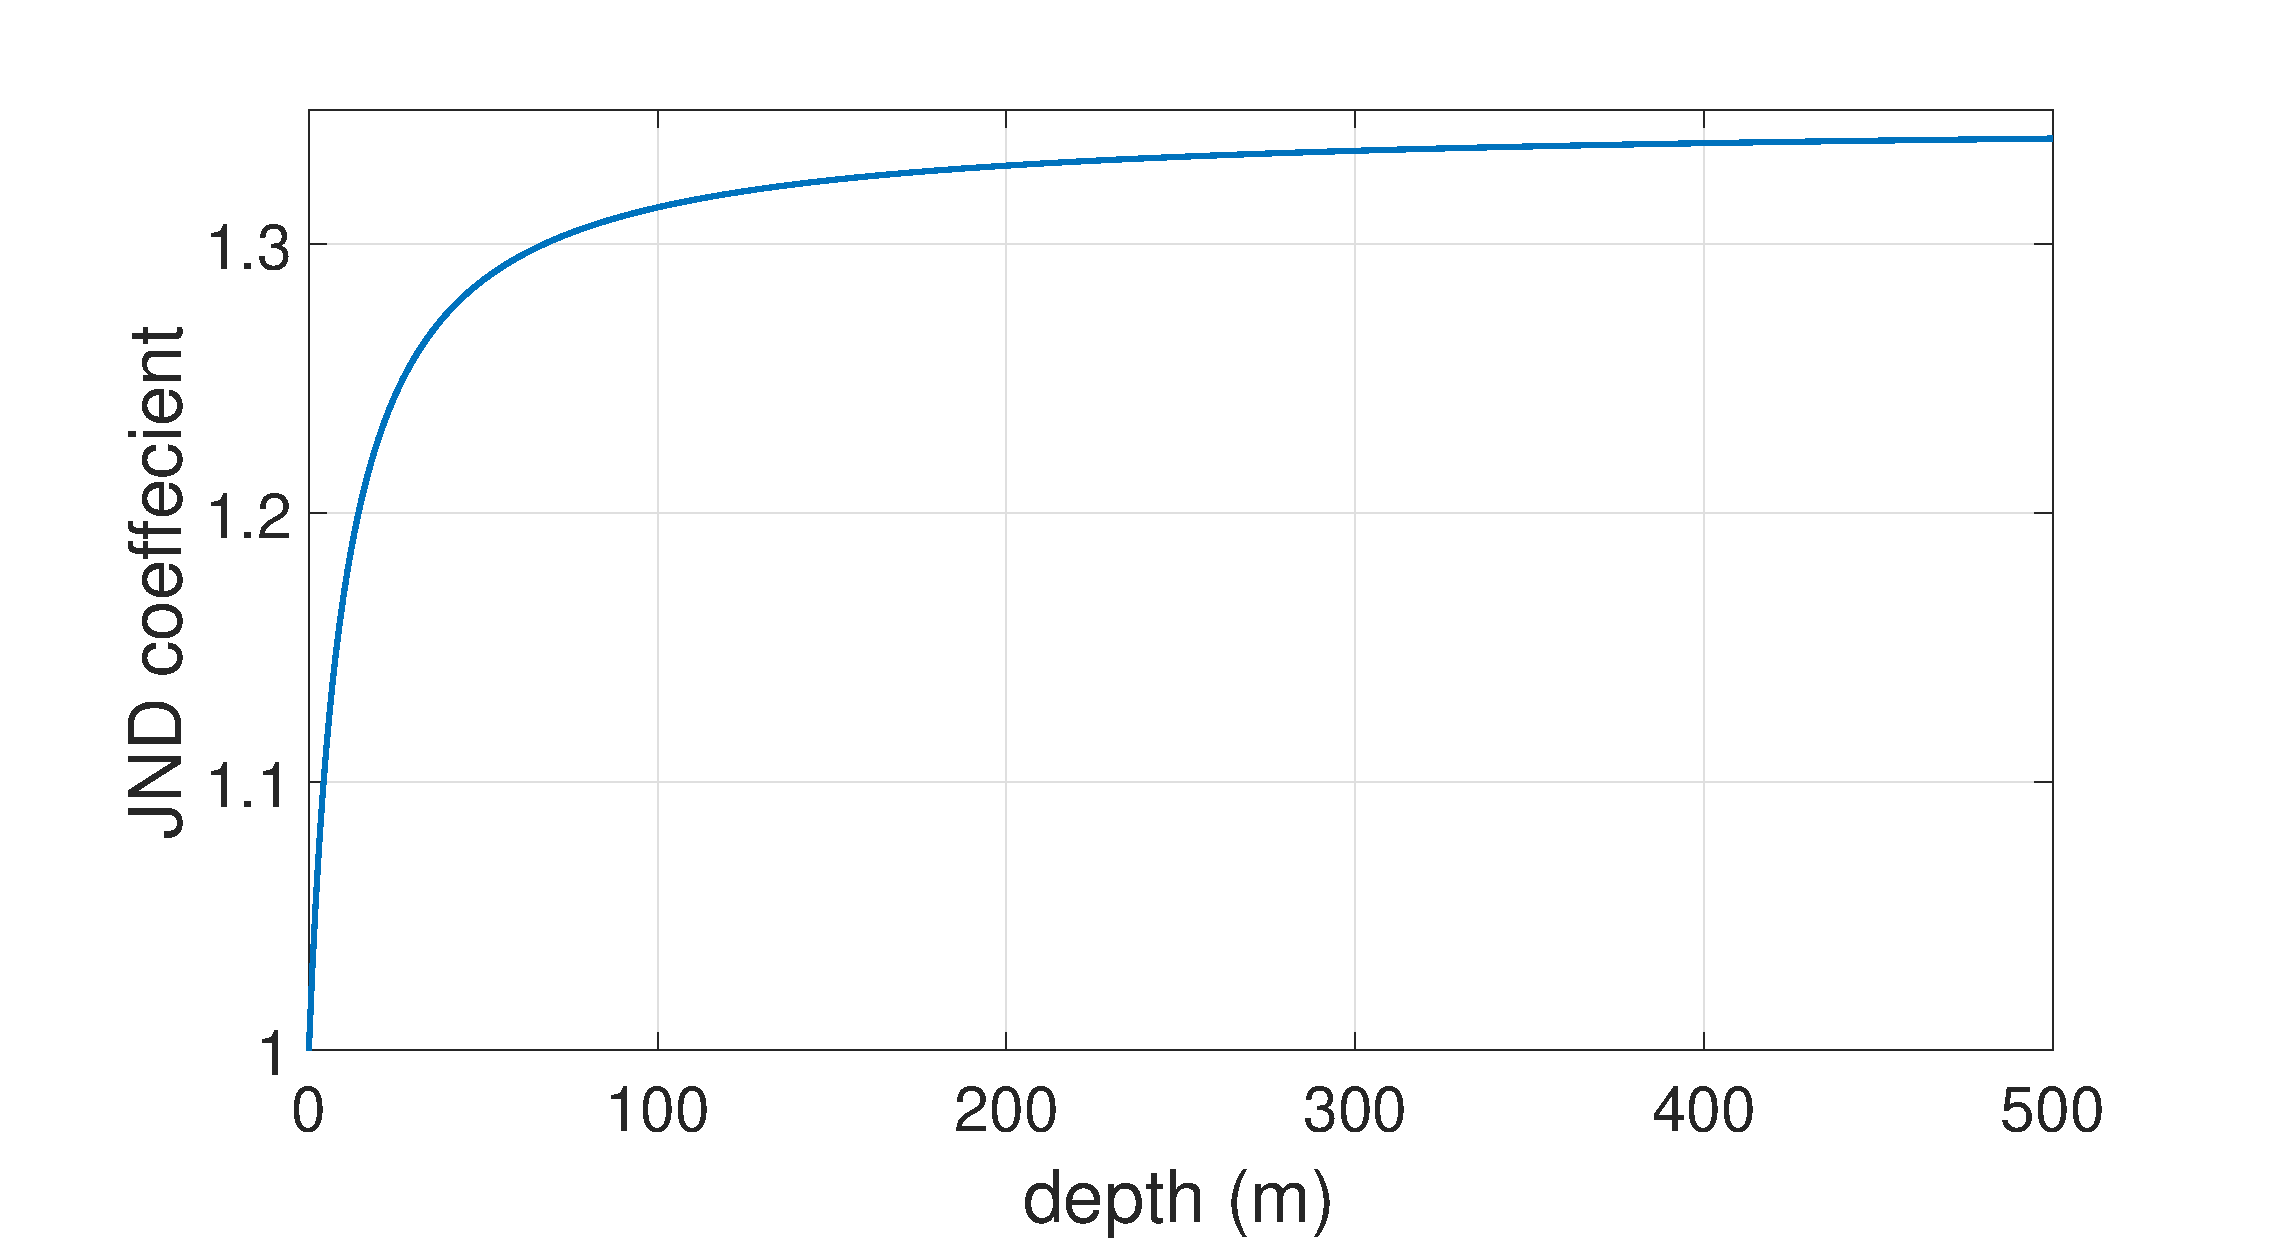
\includegraphics[width=2.5in]{images/JNDdof.eps}
  \caption{$f_{DoF}(D)$, the JND coefficient of Depth-of-Field.}
  \label{JNDdof}
  \end{figure}

\subsubsection{JND v.s. luminance \& light / dark adaptation}

In human vision system, in order to transit from day to night vision they must undergo a dark adaptation period in which each eye adjusts from a high luminescence setting to a low luminescence setting. (\cite{darkadaptation}, \cite{darkadaptation2}) Similarly, when human eyes transit from night to day vision they also undergo a light adaptation period. It is well-known that during the process of light / dark adaptation, human visual acuity decreases.

In non-VR video displays, the environment illumination totally depends on the real environment (e.g. under the sunlight, or in a classroom with electric lamp, or in a dark room). However, VR video displays are very different. When user wears HMD, the environment illumination totally depends on video content itself. So when the illumination of video content changes dramatically, eyes need a period of time to adapt the new illumination.

Fig. \ref{JNDadapt-lum} shows $JND_{lum\&ada}(l, \Delta e)$, the combined effect of light / dark adaptation and content luminance to JND. $l$ represents content luminance, $\Delta e$ represents the variation of environment luminance before the test and during the test. 

Be similar to above 2 results, this combined effect can also be decoupled into 2 parts:

\begin{figure}
  \centering
  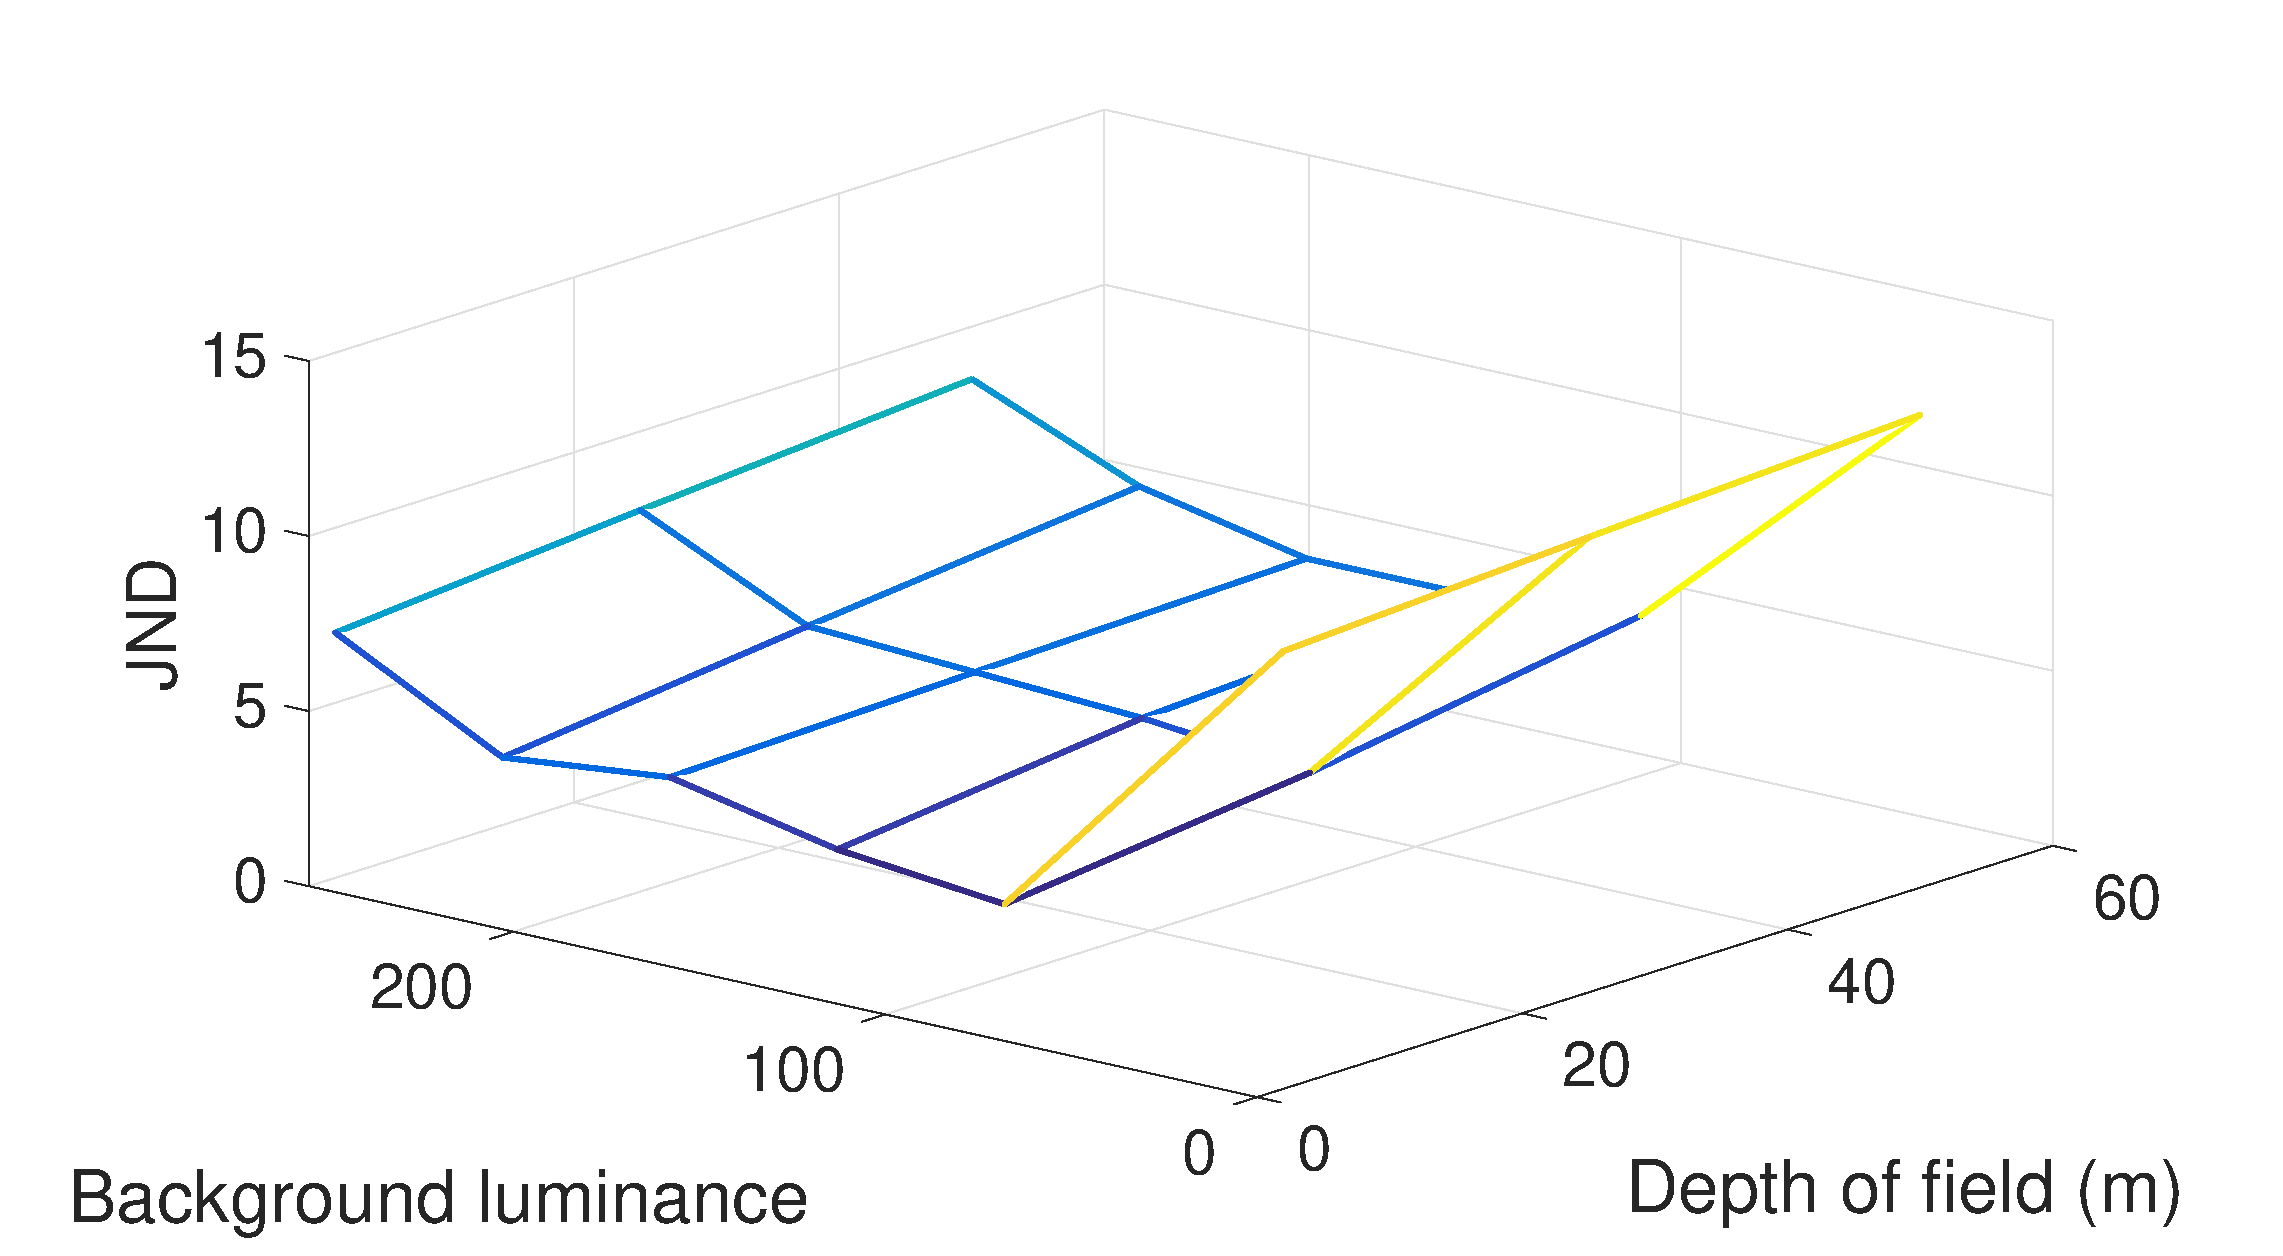
\includegraphics[width=2.5in]{images/JNDdof-lum.eps}
  \caption{JND due to content luminance and Depth-of-Field.}
  \label{JNDadapt-lum}
  \end{figure}

\begin{alignat}{2}\
JND_{lum\&ada}(l, \Delta e) = f_{lum}(l) \times f_{adapt}(\Delta e)
\end{alignat}

where $f(_{lum}(l))$ represents the visibility threshold with only consideration of content luminance, and $f_{adapt}(\Delta e)$ is a coefficient which represents DoF's influence on visibility threshold.

And we obtain $f_{adapt}(\Delta e) = \frac{JND_{lum\&ada}(l, \Delta e)}{f_{lum}(l)}$ as Fig. \ref{JNDadapt}.

\begin{figure}
  \centering
  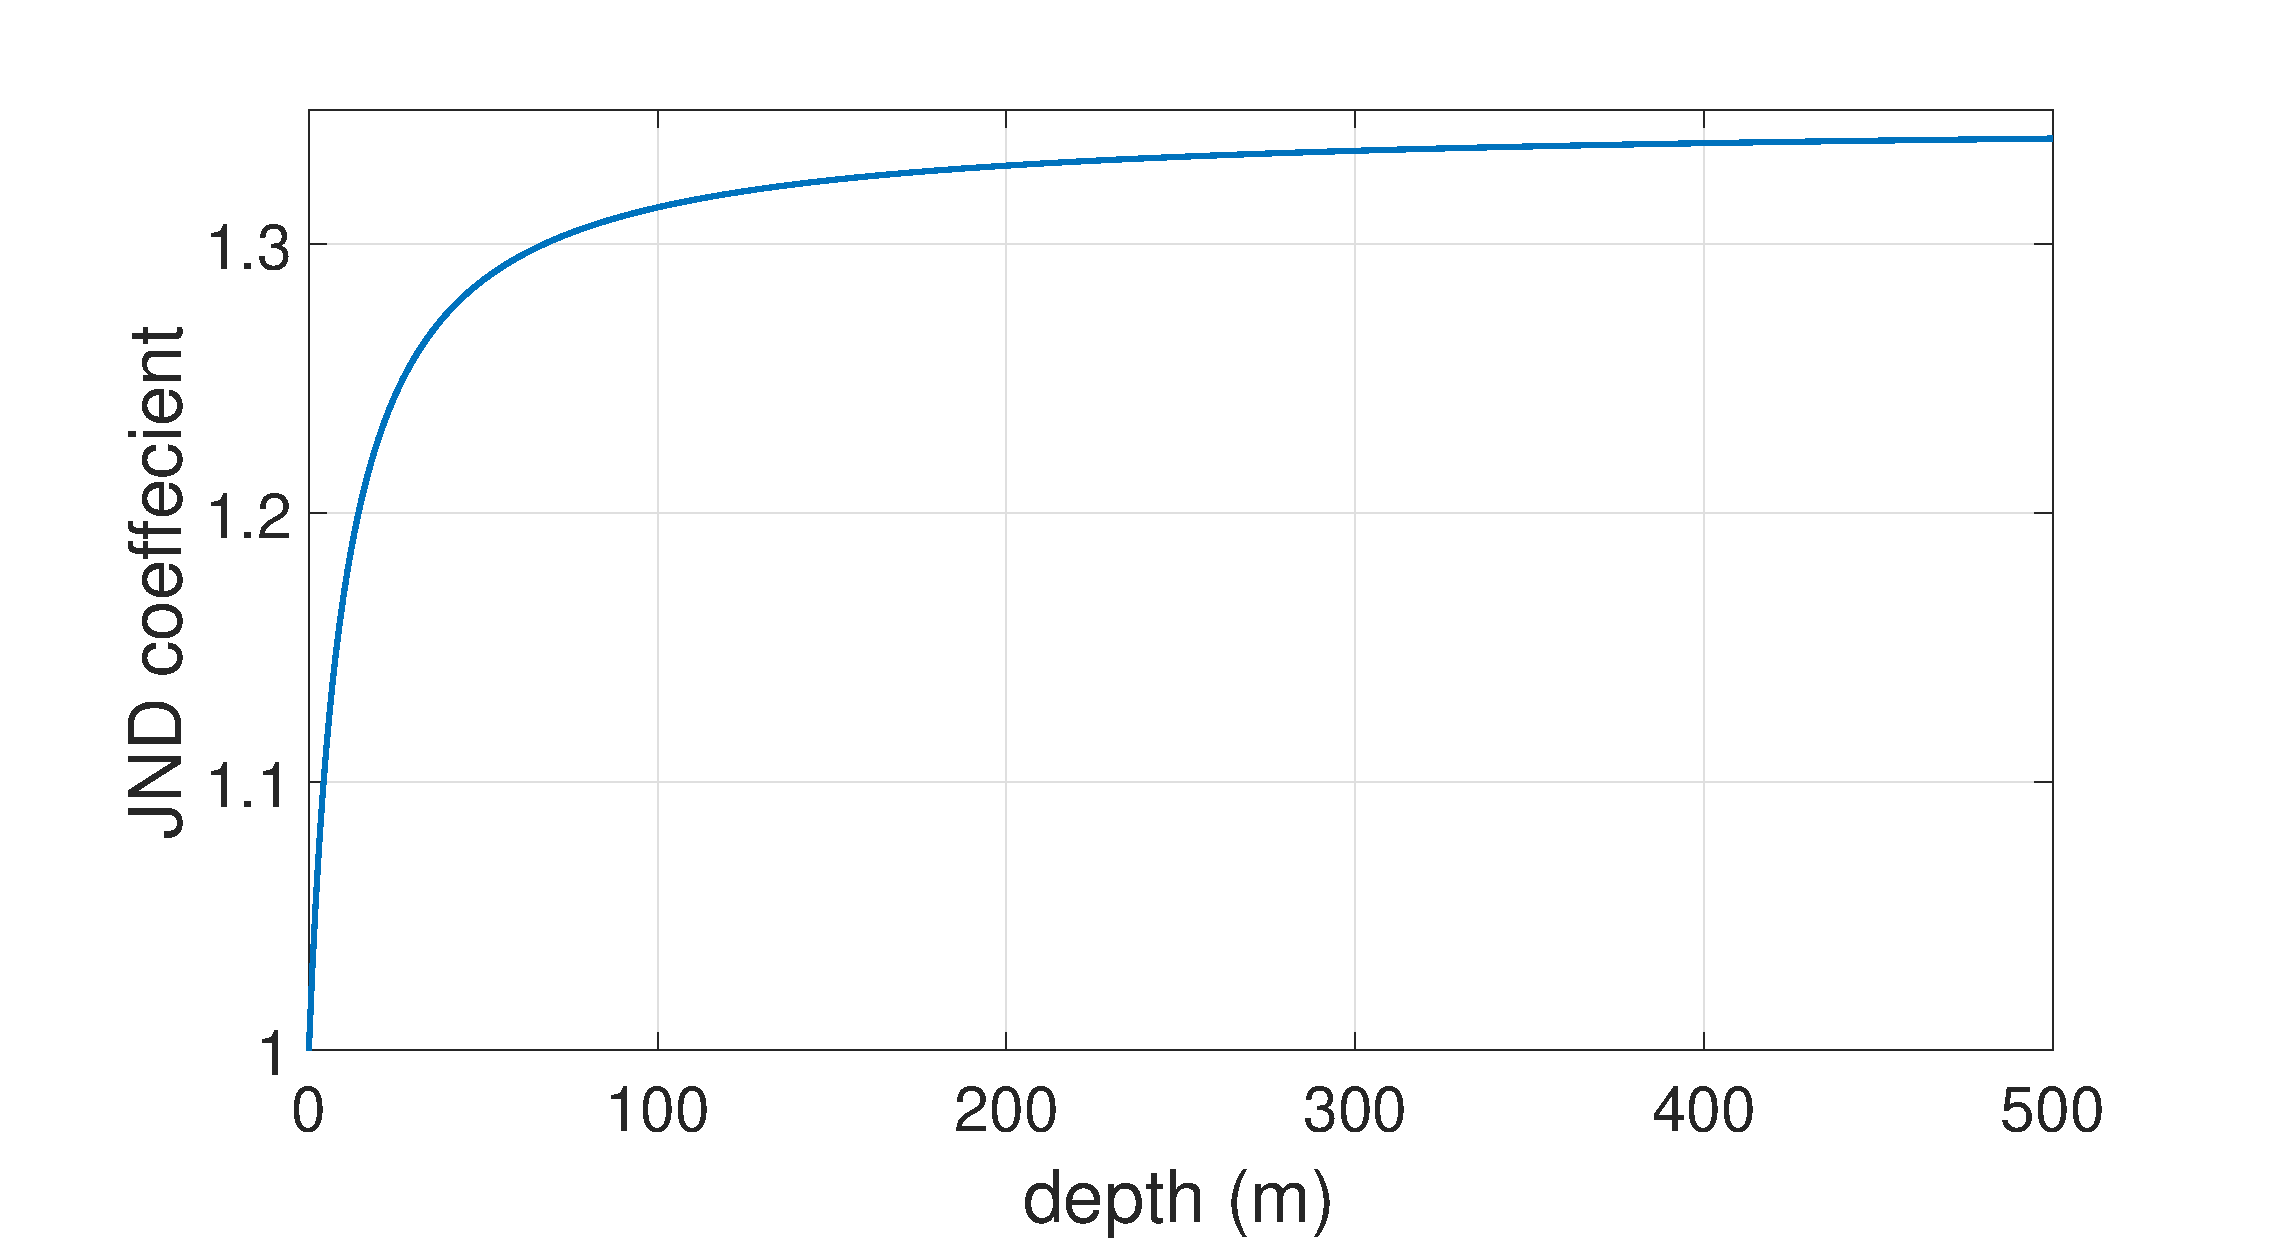
\includegraphics[width=2.5in]{images/JNDdof.eps}
  \caption{$f_{adapt}(\Delta e)$, the JND coefficient of light / dark adaptation.}
  \label{JNDadapt}
  \end{figure}

\subsubsection{Put it together}

To get the final JND value, we need to put traditional JND factors together with above three new VR-only JND factors. 

Table \ref{table2} lists the symbol and definition used for JND computation.

\begin{table}[h]
\centering
\caption{symbol and definition used for JND computation}\label{table2}
\begin{tabular}{|p{1.5cm}|p{4cm}|p{1.5cm}|}
\hline
symbol & Definition & Source\\
$f_{lum}(l)$ & Visibility threshold due to content luminance $l$. & \cite{PSPNR}, \cite{luminance1}\\
$f_{text}(t)$ & Visibility threshold due to texture complexity $t$. & \cite{PSPNR}\\
$f_{dist}(d)$ & The coefficient of viewpoint-object distance $t$. & \cite{distance}\\
$f_{track}(v), f_{notrack}(v)$ & The coefficient of viewpoint moving speed $v$. & This paper\\
$f_{DoF}(D)$ & The coefficient of Depth-of-Field $D$. & This paper\\
$f_{adapt}(\Delta e)$ & The coefficient of light / dark adaptation $\Delta e$. & This paper\\
\hline
\end{tabular}
\end{table}

For the first 3 JND factors which have been well-studied in traditional video display, measurement of $f_{lum}(l)$ can be found in \cite{luminance1}, measurement of $f_{text}(t)$ can be found in \cite{PSPNR} and measurement of $f_{text}(t)$ can be found in \cite{distance}. We leave the detail of their computation out of this paper.

It is widely accepted \cite{PSPNR} that in non-VR video display, $JND_{nonVR}$ can be computed as follow:

\begin{alignat}{2}\
JND_{nonVR} = \max \{ f_{lum}(l) , f_{text}(t)\} \times f_{dist}(d)
\end{alignat}

Since we have proved that in VR display, 3 new VR-only JND factors, viewpoint moving speed, DoF, light / dark adaptation can be regarded as coefficient on non-VR JND value, $JND_{VR}$ can be computed as:

\begin{alignat}{2}\
JND_{VR} = \max \{ f_{lum}(l) , f_{text}(t)\} \times f_{dist}(d) \times f_{track/notrack}(v) \times f_{DoF}(D) \times f_{adapt}(\Delta e)
\end{alignat}

\section{Object-based tiling scheme}

In this section we first introduce our object detection method. Based on this object detection, we describe our object-based tiling scheme and make comparison with state-of-art grid-like tiling schemes.

\subsection{Object Detection based on Quality-Bitrate Efficiency}

In the field of computer vision, there are many object detection algorithms which can cut a video into different content objects. However, in our video tiling scheme, the purpose of object  detection is little different. Actually we do not care if two adjacent tiles contain exactly the same object or they contain different objects. The most important thing is the probability of them to be allocated the same bitrate level by client. Even though two adjacent objects are different, if they have similar properties (like luminance, contrast, Depth of Field), we can also contain them in one tile because there is high probability for user to allocate them the same bitrate level.

To meet our purpose, for any rectangular tile which can be independently encoded, we define its \textbf{Quality-Bitrate Efficiency (QBE)} as follow:

\begin{alignat}{2}\
QBE = \frac{PSPNR_{highest} - PSPNR_{lowest}}{B_{highest} - B_{lowest}} \label{QBE}
\end{alignat}

where $PSPNR_{highest}$ / $PSPNR_{lowest}$ denotes the PSPNR value of this tile's highest / lowest bitrate version, and $B_{highest}$ / $B_{lowest}$ denotes the bitrate of this tile's highest / lowest bitrate version. In order to eliminate the influence for PSPNR by different user viewpoint positions, we only consider luminance, texture complexity and Depth-of-Field in QBE computation. These informations can be obtained completely on server-side.

In a video frame, different objects have different QBE. QBE is highly related to properties of content objects. According to PSPNR computation (Section 4), objects with very dark / light object luminance, complex texture or high depth of field, usually has higher QBE.

In perceived quality optimization, it is obvious that objects with high QBE is more likely to be allocated high bitrate (because it can improve more PSPNR in the same bandwidth cost), and objects with low QBE is more likely to be allocated low bitrate. So when two adjacent objects have similar QBE, they have high probability to be allocated the same bitrate level. 

\subsection{Tiling video by objects}

Based on above insights, we aim to cut the video into $T$ rectangular tiles of unequal size, such that content items within the same tile have similar QBE.

In this paper, tiling video by objects consists of 3 steps:

\textbf{Step 1: Partitioning the original video into 12*24 rectangular basic units of equal size.} 

Basic unit is the smallest unit of proposed object-based tiling. In the tiling process, each tile must be composed by one or several entire basic units which form a rectangular shape.

\textbf{Step 2: Computing QBE of each basic unit.}

We get QBE of each basic unit according to (\ref{QBE}). After that, suppose a tile $t$ consists of $N_t$ basic units $u_1$, $u_2$, ... , $u_{N_t}$ , we can compute its QBE Variance ($QBEV_t$) as follow:

\begin{alignat}{2}\
QBEV_t = \frac{\sum_{1 \le i \le N_{t}}{(QBE_{u_i} - E(QBE_{u_{i}}))^2}}{N_t}
\end{alignat}

where $E(QBE{u_i})$ is the average QBE of basic units in tile $t$:

\begin{alignat}{2}\
E(QBE_{u_i}) = \frac{\sum_{1 \le i \le N_{t}}{QBE_{u_i}}}{N_t}
\end{alignat}

A tile with high QBEV means visual properties (e.g. luminance, texture complexity) of objects in this tile have very different properties. A tile with low QBEV means objects in this tile are similar. So a good tiling scheme should keep each tile's QBEV value as low as possible.

\textbf{Step 3: Merging all basic units into T rectangular tiles, such that their weighted average QBEV is minimal.}

Suppose $V$ is the whole video frame. $R_i$ is the $i$th rectangular tile and $S_i$ is its area.This optimization problem can be formalized as following:

\begin{equation}
\begin{aligned}
\min \sum_{i = 1}^T QBEV_{i} S_i \hspace{3cm} \\
\text{s.t.} \bigcup _{i=1}^N R_{i} = V\hspace{3cm} \\
R_i \bigcap R_j = \emptyset \hspace{1cm} \forall 1 \le i, j \le T
\end{aligned}
\end{equation}

However, this optimization problem is a NP-hard problem, so we can not get the optimal solution in polynomial time. In practice, we apply a dynamic programming algorithm to get the suboptimal solution for this problem. In our implementation, we set $T = 72$ since it performs well in most situations.

\subsection{Comparison of object-based tiling and grid-like tiling}

We evaluate our tiling scheme and make comparison with traditional grid-like tiling schemes.

Fig. \ref{tiling} shows the PSPNR-bandwidth tradeoff of 3*6 grid tiling, 6*12 grid tiling, 12*24 grid tiling and proposed object-based tiling. 

  \begin{figure}
  \centering
  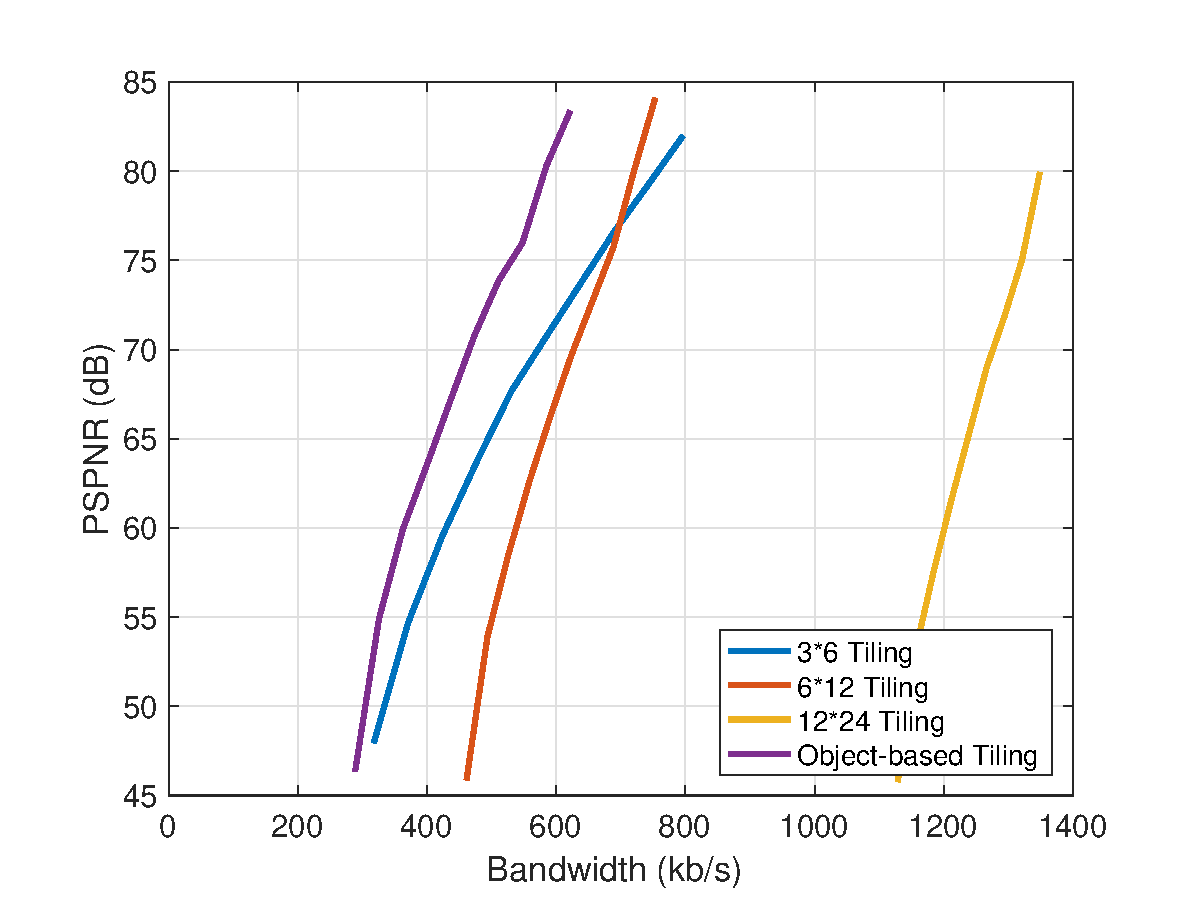
\includegraphics[width=2.5in]{images/tiling.eps}
  \caption{The PSPNR-bandwidth tradeoff of proposed Object-based Tiling scheme and traditional grid-like tiling scheme (3*6, 6*12 and 12*24).}
  \label{tiling}
  \end{figure}

For traditional gird-like tiling schemes, the performance of different tiling granularity depends on bandwidth. In low bandwidth, most part of video is allocated the lowest bitrate level. So there is no need to cut the video into many tiles. 3*6 tiling performs well because of its high bitrate efficiency. However, in high bandwidth, a coarse tiling granularity causes suboptimal bitrate allocation, so it is beaten by 6*12 tiling. Unfortunately, 12*24 tiling performs poorly in all bandwidth because of its serious bitrate efficiency problem.

Proposed object-based tiling scheme beats traditional grid-like tiling scheme of all bandwidth. In high bandwidth situation, it saves 20\% bandwidth compared with 6*12 grid-like tiling. Although 3*6 tiling's low bandwidth performance is near to proposed object-based tiling, its high bandwidth performance is far away from object-based tiling.

\section{Client-side PSPNR computation and optimization}

In client-side PSPNR optimization, client first need to compute PSPNR value for each rate allocation. However, PSPNR computation needs information of both video content and user behavior. In practice, client is unaware of video content before actually receiving video content. How to decouple PSPNR computation process to let client-side get PSPNR value without knowing information of video content is a big challenge.

To optimize PSPNR on client-side, we first present an approximation of PSPNR computation, then we describe our algorithm of client-side PSPNR optimization.

\subsection{Client-side PSPNR computation}

First we decouple JND into Content JND (CJND) and Behavior JND (BJND). We define a pixel $(x, y)$'s Content JND (CJND) as:

\begin{equation}
\begin{aligned}
CJND(x, y) = \max \{ f_{lum}(l(x, y)) , f_{text}(t(x, y))\} \times f_{DoF}(D(x, y)) \label{CJND}
\end{aligned}
\end{equation}

CJND is only related to video content. It can be pre-computed on server-side.

We define Behavior JND (BJND) as:

\begin{equation}
\begin{aligned}
BJND(x, y) =  f_{dist}(d(x, y)) \times f_{speed}(v) \times f_{adapt}(\Delta e) \label{BJND}
\end{aligned}
\end{equation}

BJND is only related to client behavior, it is totally independent from video content so it can be obtain on client-side. 

Based on (\ref{CJND}) and (\ref{BJND}), equation (\ref{original_pmse}) can be rewritten as:

\begin{alignat}{2}\
PMSE=E\{ \left[ |p(x, y) - \hat{p}(x, y)| - CJND(x, y) \times BJND(x, y)\right]^2 \times \Delta (x, y)\} \label{apprxPMSE}
\end{alignat} 

Given a tile, although the CJND value of different pixel may vary greatly, we notice that BJND value of different pixels are not so different. This is because:

 (1) All pixels in one tile share the same $f_{speed}(v)$ and $f_{adapt}(\Delta e)$. 
 
 (2) Although strictly, $f_{dist}(d(x, y))$ is different for different pixel $(x, y)$, pixels in the same tile is usually spatial adjacent. Their distance to user viewpoint is roughly the same, so they usually have similar $f_{dist}(d(x, y))$ value.

Based on above insight, we use only one BJND value in one tile, instead of one BJND value for each pixel. We suppose $(x_{mid}, y_{mid})$ is the pixel in the center of the tile, then we can approximate (\ref{apprxPMSE}) as:

\begin{alignat}{2}\
PMSE \approx E\{ \left[ |p(x, y) - \hat{p}(x, y)| - CJND(x, y) \times BJND(x_{mid}, y_{mid})\right]^2 \times \Delta (x, y)\} \label{apprx_pmse}
\end{alignat} 

Now, in (\ref{apprx}), server has all information (including $p(x, y)$, $\hat{p}(x, y)$, $CJND(x, y)$, $\Delta (x, y)$) with only exception of one single value: $BJND(x_{mid}, y_{mid})$. Moreover, according to definition of PSPNR, PSPNR is strictly monotonically increasing with $BJND(x_{mid}, y_{mid})$. So in practice, server can presuppose $N$ different BJNDs offline to compute $N$ corresponding PSPNRs by (\ref{f1}), (\ref{apprx_pmse}), (this step we call PSPNR precomputation) then transforms these PSPNR values to client-side. Client-side computes the actual $BJND(x_{mid}, y_{mid})$ value and choose the nearest presupposed BJND, then obtain the corresponding PSPNR value.(this step we call PSPNR computation)

In real-world implementation, in order to further improve PSPNR approximation accuracy, when the actual $BJND(x_{mid}, y_{mid})$ is in the gap between 2 adjacent presupposed BJNDs, we simply compute the actual PSPNR by linear regression. Fig. \ref{PSPNR_computation} shows the approximation accuracy. In 88\% situations, error rate of proposed method is less than 5\%. In realtime VR video streaming, PSPNRs of presupposed BJNDs are packaged in MPD file which can be downloaded by client, their bandwidth cost is negligible.

\begin{figure}
  \centering
  \includegraphics[width=2.5in]{images/PSPNR_computation.eps}
  \caption{CDF of PSPNR approximation accuracy.}
  \label{PSPNR_computation}
  \end{figure}

\subsection{PSPNR optimization}

Client-side PSPNR optimization consists of 2 levels:

\emph{Level 1:} In constraint bandwidth consumption and buffer size, allocate the bitrate of each temporal segment.

\emph{Level 2:} For each temporal segment, after its bitrate is allocated, distribute the bitrate to each spatial tile.

\subsubsection{Level 1: Allocating bitrate of each temporal segment}

Suppose a VR video consists of $K$ temporal segments: $s_1$ , $s_2$, ... , $s_K$. For segment $s_k$, when it is allocated $R_k$ bandwidth, it can obtain $q_{k}(R_k)$ PSPNR. Our problem is to allocate bitrate $R_1$, $R_2$, ... , $R_K$ for each temporal segment.

When the client is allocating bitrate for video segment $s_k$, suppose the buffer status is $B_k$ and the bandwidth throughput prediction is $C_k$. Moreover, the previous video segment $s_{k-1}$ has been allocated the bitrate $R_{i-1}$, thus its perceived quality is $q_{k-1}(R_{k-1})$. In rate adaptation logic, making decision of $R_k$ should take consideration of these values (\cite{BOLA}, \cite{MPC}) to avoid rebuffing and quality fluctuation.

Then the rate allocation problem can be formalized as:

\begin{equation}
\begin{aligned}
R_k = f(q_{k-1}(R_{k-1}), B_k, C_k)
\end{aligned}
\end{equation}

Fortunately, BOLA (Near-Optimal Bitrate Adaptation for Online Videos) \cite{BOLA} is a well-known method to solve the problem completely on client-side, and it has been well built in Dashjs. Given the value of $R_{i-1}, B_i, C_i$, the algorithm output an appropriate $R_i$. So BOLA can be directly applied on the Level 1 rate allocation. We leave the detail of BOLA design out of this paper since there are plenty of works about BOLA design in rate adaptation.

\subsubsection{Level 2: Allocating bitrate of each spatial tiles}

In above Level 1 rate allocation, two questions are remained: (1) Given rate allocation $R_k$ for temporal segment $s_k$, how to allocate the bitrate to each tile in segment $s_k$. (2) How to build $q_k(R_k)$, the mapping from bitrate to PSPNR. 

Actually, the second question can be merged into the first question: For a temporal segment $s_k$, when the bitrate of each tile is determined according to $R_k$, its PSPNR $q_k(R_k)$ is determined. So the problem of Level 2 rate allocation is how to distribute $R_k$ bitrate to each tile to optimize $q_k(R_k)$.

According to (\ref{f1}), PSPNR is monotonous decreasing with PMSE. Maximizing PSPNR is equivalent to minimizing PMSE.

Suppose we separate the video segment $s_k$ into $N_k$ spatial tiles, numbered 1, 2, ..., $N_k$. They are encoded into $M$ quality levels with different bitrate. We define $r_{i, j}$ as bitrate of chunk $i$ with level $j$. We define the optimal quality level for $i$-th tile as $l_i$ and define PMSE value of tile $i$ with $j$th bitrate as $p_{i, j}$.

Therefore, at each adaptation step, the client needs to solve the following optimization problem to minimizing PMSE:

\begin{equation}
\begin{aligned}
\min_{l: l_i \in [1, M]} \text{~~~~~~} & \text{~~~~} \sum_{i = 1}^N p_{i, l_i} \\
\text{s.t.} \text{~~~~} & \text{~~~~}\sum_{i=1}^N r_{i,l_i} \le R_kW.
\end{aligned}
\end{equation}

\begin{algorithm}[t]
\caption{ PSPNR driven Rate Allocation Algorithm.}
\label{alg:Framwork}
\begin{algorithmic}[1]
\Require
Throughput bound, $R_k$;
Number of tiles, $N_k$;
Number of rates, $M$;
Rate set, $\{r_{i,j}\}$;
PMSE set, $\{p_{i,j}\}$;
\Ensure
Allocation rate levels set, $\{l_i\}$;
\State Initialize knapsack revenue table $\mathcal{K}\in \mathbb{R}^{(N_k+1)\times R_k}$ by 0;
\State Construct the prefix table $\mathcal{P}\in \mathbb{Z}^{(N+1)\times R_k}$;
\For {$i$ from 1 to $N_k$}
  \For {$b \in [0,B]$}
    \State $\mathcal{K}_{i,b} = \min_{j\in[1,M]}\{\mathcal{K}_{i-1,b-r_{i-1,j}} + p_{i-1,j}\}$;
    \State $\mathcal{P}_{i,b} = \arg\min_{j\in[1,M]}\{\mathcal{P}_{i-1,b-r_{i-1,j}} + p_{i-1,j}\}$;
  \EndFor
\EndFor
\State Find $\hat{R_k}$ = $\arg\min_{b\in [0,R_k]} \{\mathcal{K}_{N_k,b}\}$;
\For {$i$ from $N_k$ to 1}
  \State $l_i = \mathcal{P}_{i,\hat{R_k}}$;
  \State $\hat{R_k} = \hat{R_k} - r_{i,l_i}$;
\EndFor \\
\Return $\{l_i\}$
\end{algorithmic}
\end{algorithm}

This optimization problem can be solved as a Multiple-Choice Knapsack problem. A brute force search which exhaustively evaluates all combinations guarantees an optimal solution. However, the computational complexity is O($N^M$). To reduce the computation time, we use a dynamic programming method (algorithm 1) to approximate the problem where the computational complexity is O($R_kMN$).

\section{Implementation}

PQVRS is open source (10K lines of code across C++, Matlab, Java, and python) and can be accessed at \cite{github}. Implementation of PQVRS is shown in Fig. \ref{implementation}. Compared with traditional video streaming system, several modules are newly added or modified, which are highlighted by pink color.

\begin{figure}
  \centering
  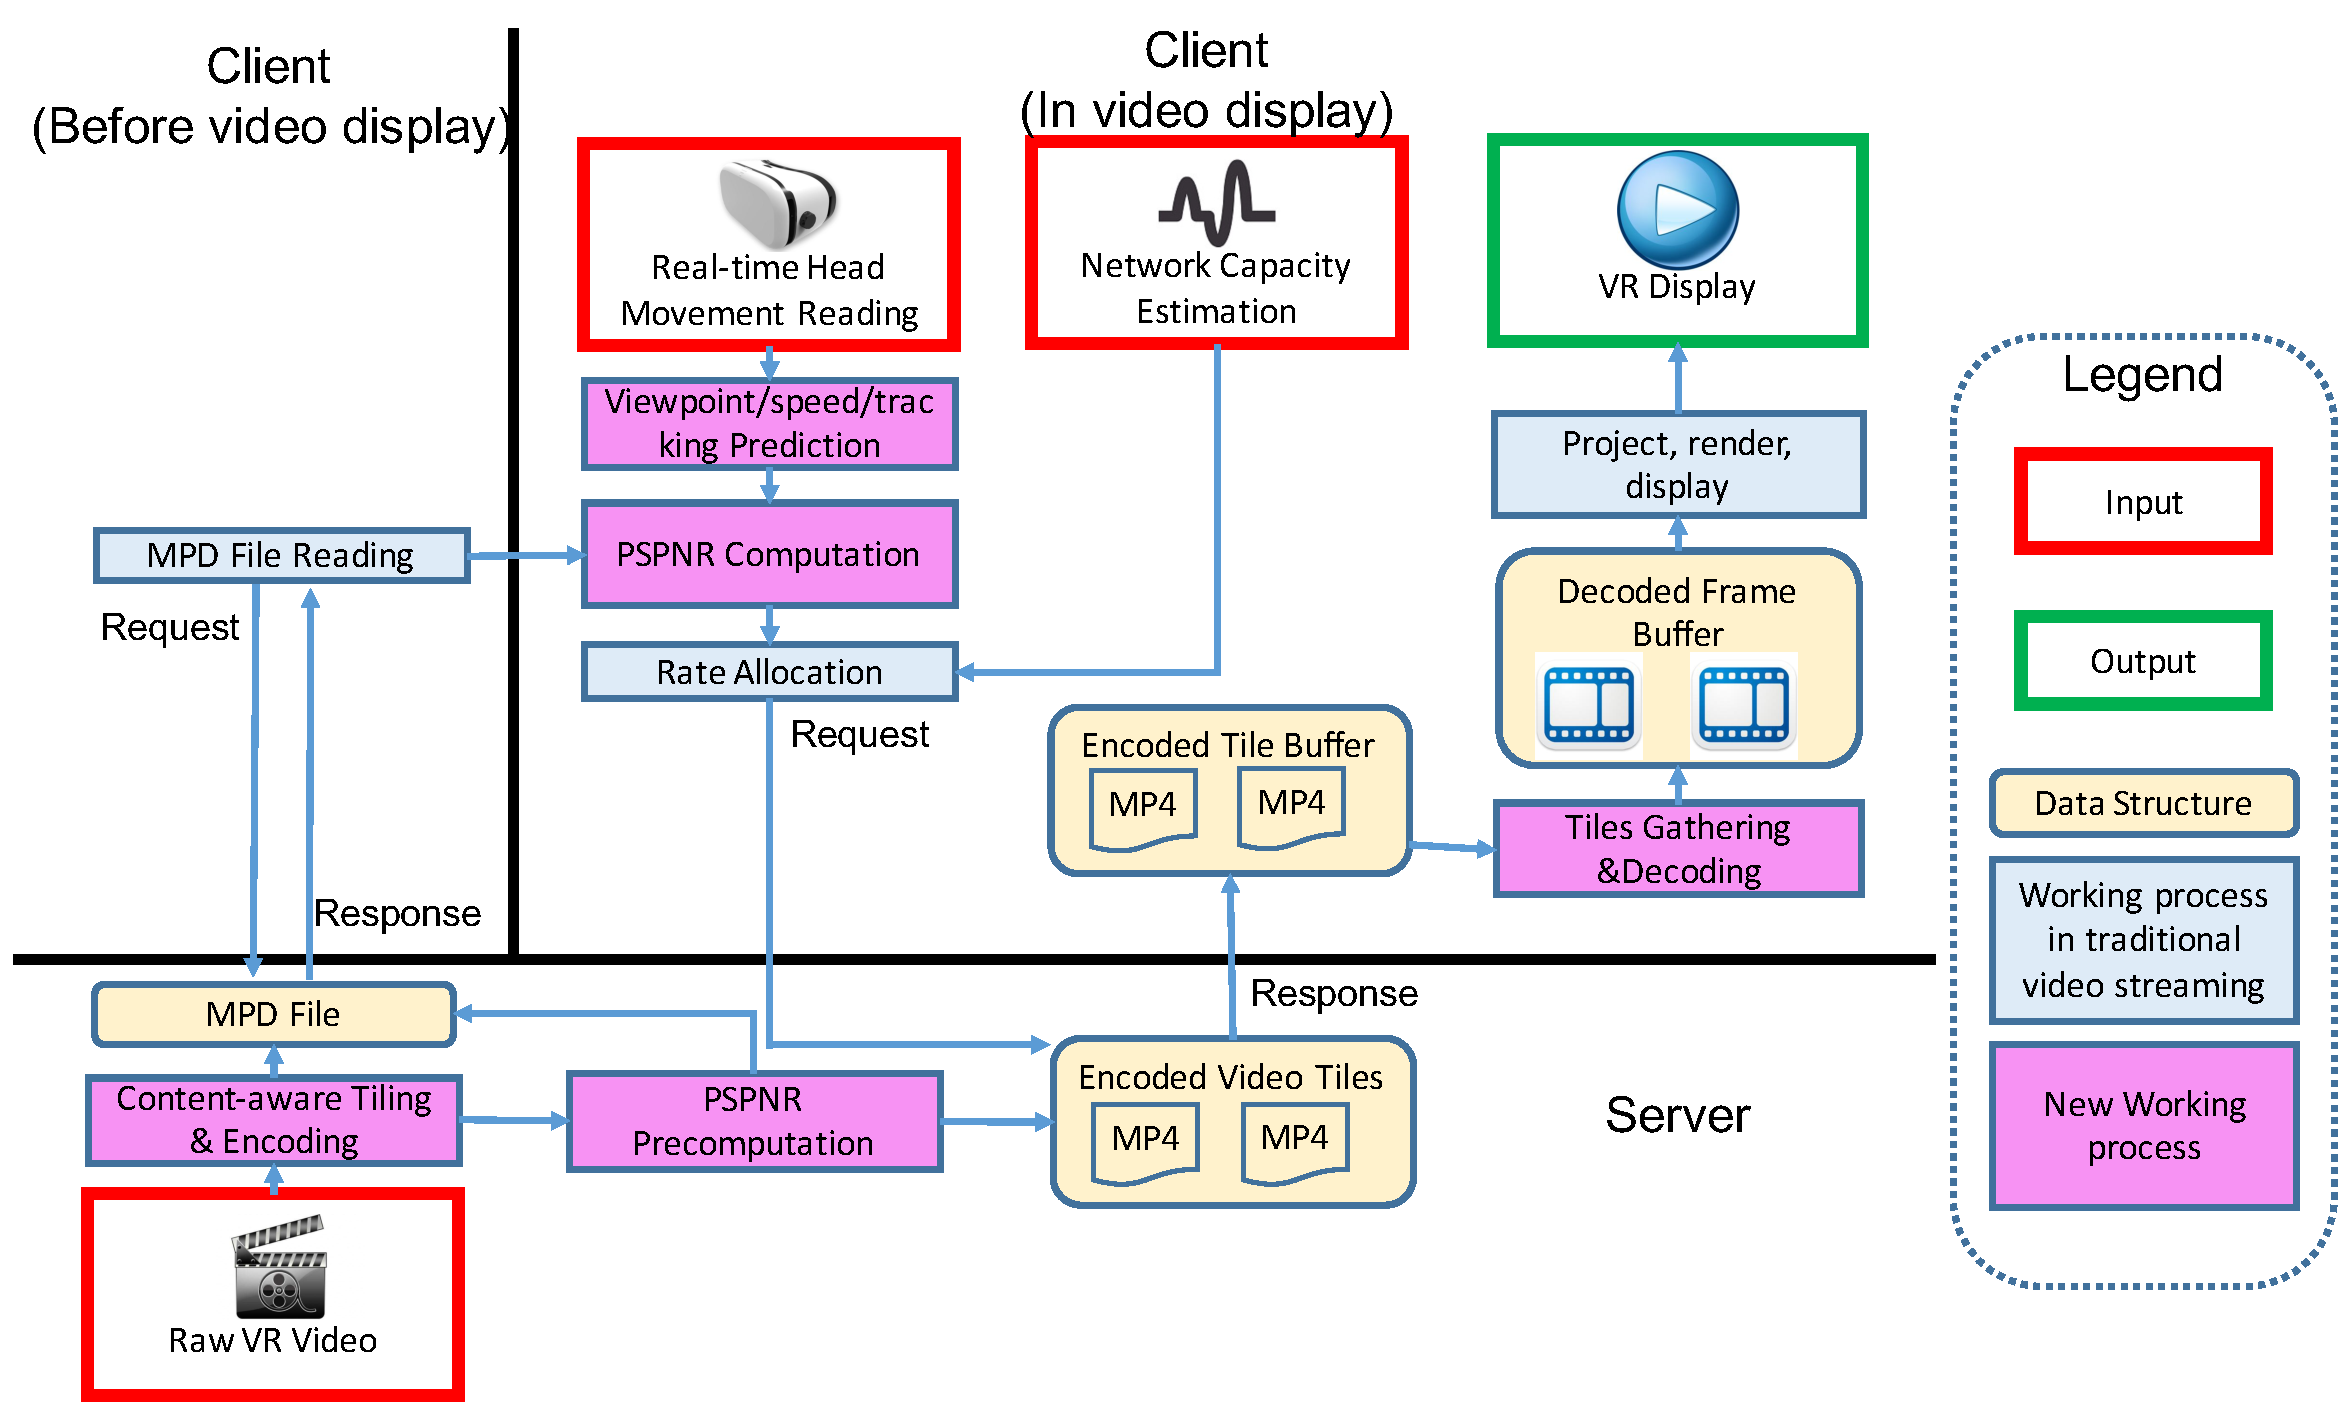
\includegraphics[width=3.5in]{images/implementation.pdf}
  \caption{Workflow of PQVRS.}
  \label{implementation}
  \end{figure}

\subsection{Server-Side}

\textbf{Content-Aware Tiling / Encoding:} Based on our tiling algorithm described in Sec. 5, we cut each video segment into $N = 72$ rectangular tiles with different size. Each tile is encoded independently. The information of tiling result is packeted into MPD file so that client is aware of how each segment is cut. In addition, with consideration of client-side decoding overhead, we encode the lowest quality version of whole video without tiling, called "Base Layer". For each video segment, we first transfer the Base Layer to client, and then transfer tiles only in user's viewport with corresponding quality. This can significantly reduce the number of tiles decoded on client-side (from 72 to around 12 per video segment), thus make PQVRS applicable on real-world devices.

\textbf{PSPNR Precomputation:} Based on equation (x), server tries to compute PSPNR of each tile for 5 different BJNDs, then packet the result into MPD file. Compared with video content, size of this additional information is negligible.

\subsection{Client-Side}

\textbf{Viewpoint / Speed / Tracking prediction:} In our system, viewpoint prediction is achieved by linear regression because of its efficiency and robustness. According to result of viewpoint prediction, we can estimate user's viewpoint moving speed by differentiating adjacent user viewpoints. Moreover, since we have analyzed object traces of video on server-side by YOLO \cite{yolo} and deliver the brief description to client-side, client-side can match the predictive viewpoint traces and object traces in order to predict if user is going to tracking an object.

\textbf{PSPNR Computation:} On client-side, based on our viewpoint / speed / tracking prediction, the value of BJND can be obtained by equation (x). Then client read MPD file to get the PSPNR results with different BJNDs, and choose the one with the nearest BJND.

\textbf{Tiles Gathering \& Decoding:} For each video segment, client first decode the Base Layer. For tiles in user's viewport, we set up a multi-process decoder based on ffmpeg, and set up a buffer to cache the decoded frames of tiles to be played in the future. Specifically, the decoding scheduler dynamically selects a received tile and sends it to an idle decoder. The decoded frames are not necessarily consumed right away; instead they can be stored in the buffer residing in the video memory. When a cached frame is needed during the playback, its corresponding tiles are fed into GPU, then then mapping them from 2D to 3D for rendering on Head-Mounted Device.
\section{Performance Evaluation}

In this section, we show that:

\begin{itemize}

\item In the network with fixed bandwidth, compared with state-of-the-art VR streaming system, PQVRS saves 45\% bandwidth on average while providing the same PSPNR, or provides 15-20 higher PSPNR in the same bandwidth.

\item In the network with unstable bandwidth, PQVRS improves 10 higher PSPNR and decreases 50\% stalling.

\item In real-world perceived quality rating by users, PQVRS can obtain better user rating.

\item Improvement analysis shows that PQVRS has substantial improvement on ... video segments, and has marginal improvement on ... video segments.

\end{itemize}

\subsection{Evaluation Setup}

To evaluate the performance, we implement PQVRS, a real-world VR streaming system which adaptively choose the quality of each part of video and display on HMD. Fig. \ref{network} shows the network topology in the experiment, which consists of a client and a server.

\begin{figure}
  \centering
  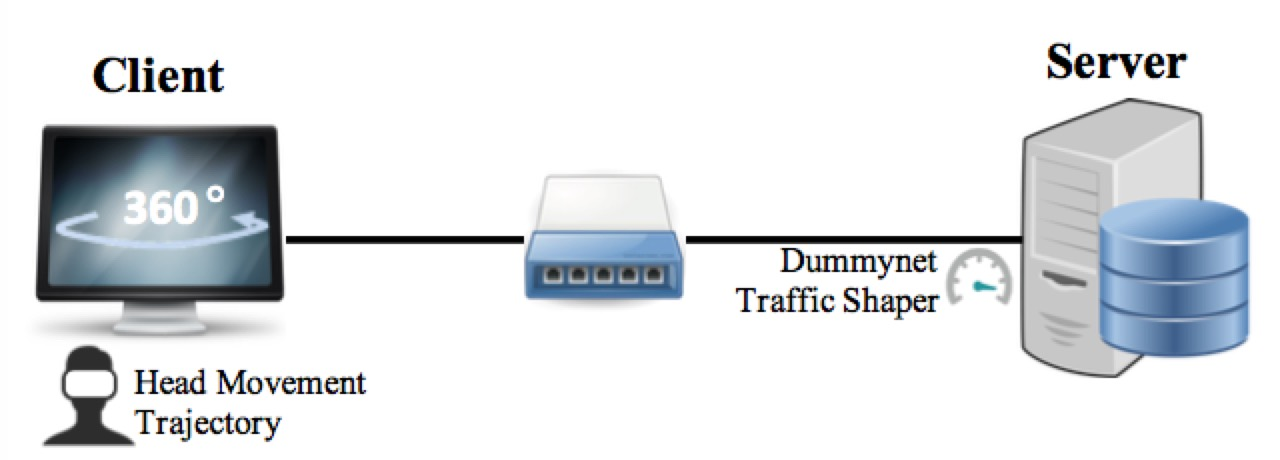
\includegraphics[width=3in]{images/network.jpg}
  \caption{Network topology.}
  \label{network}
  \end{figure}

In the experiments, we choose 50 videos with different types and lengths. We set the duration of one video segment as 1 second. To generate different quality videos, we use quantization parameter (QP) ranging from 22 to 42 in steps of five leading to five different bitrate versions. 

In our experiment, 3 VR streaming systems are chosen to make comparison:

\begin{itemize}

\item \emph{Flare \cite{Flare}:} A state-of-the-art viewpoint-driven VR streaming. Video is cut into 4*6 spatial rectangular tiles. Tiles on user's viewpoint is allocated the high bitrate. For other tiles, bitrate is allocated linearly decreasing with its distance to user's viewpoint.

\item \emph{PQVRS-:} Video is cut into 6*12 spatial rectangular tiles. With consideration of user viewpoint, content luminance and texture complexity, we do adaptive streaming to maximize user-perceived quality.

\item \emph{PQVRS:} Our proposed method in this paper. Object-based video tiling is used to cut video into tiles with different size. Besides user viewpoint, content luminance and texture complexity, we also take consideration of viewpoint moving speed, content Depth-of-Field and light / dark adaptation, and do adaptive streaming to maximize user-perceived quality.

\end{itemize}

\subsection{Performance comparison under fixed bandwidth}

When network is under a fixed bandwidth, video streaming is stalling-free since the requested video segment will always be retrieved back to client on time. User perceived quality is almost only related to PSPNR. So we test the PSPNR-bandwidth tradeoff for above methods under fixed bandwidth. Fig. \ref{practical_imp} shows the result.

  \begin{figure}
  \centering
  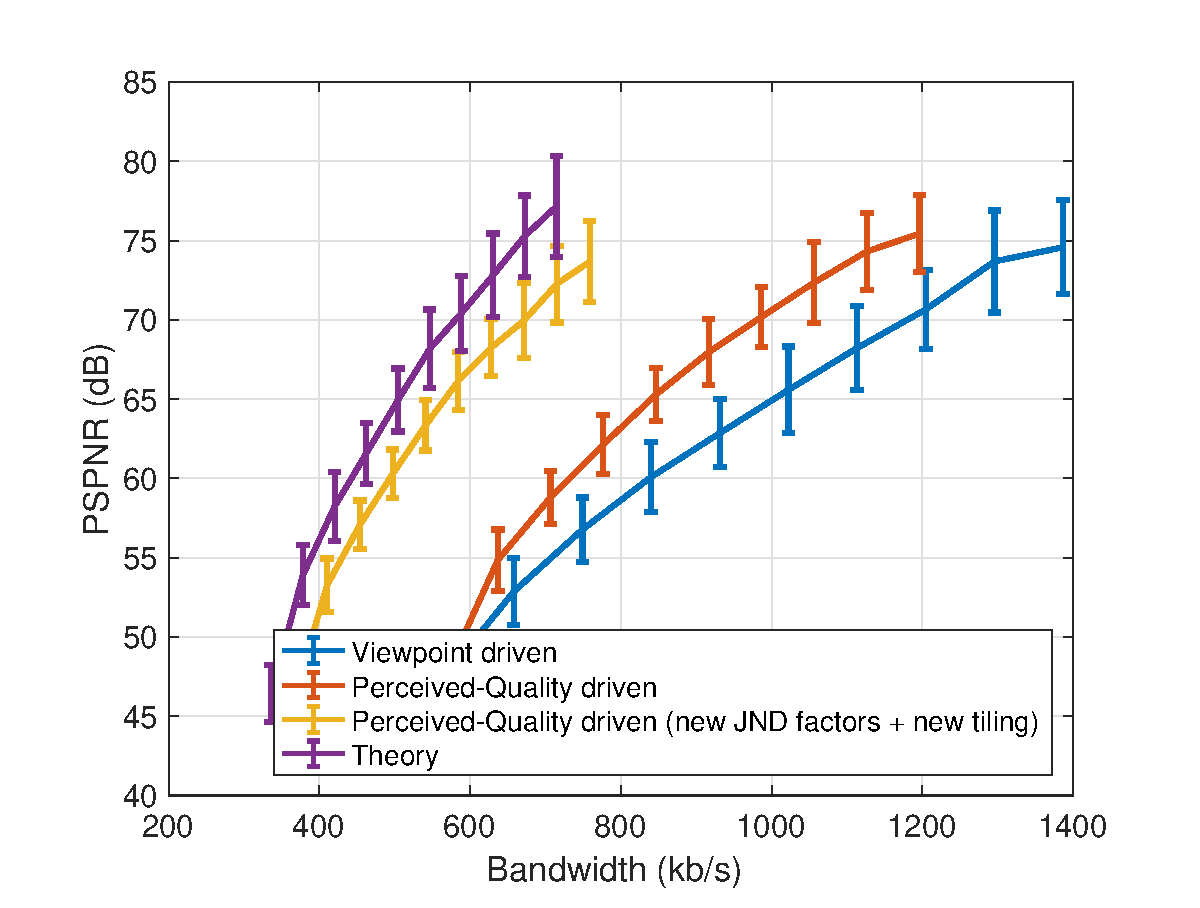
\includegraphics[width=3in]{images/practical_improvement.eps}
  \caption{PSPNR-bandwidth tradeoff of 4 methods: Viewpoint-driven, PQVRS-, PQVRS, theoretical performance.}
  \label{practical_imp}
  \end{figure}

\textbf{Key observations:}

\subsection{Performance comparison under real-world bandwidth}

Actually, in real-world video streaming, bandwidth is unstable which may change significantly in a short time. When the bandwidth change dramatically from a high level to a low level, it not only decrease the value of PSPNR, but also causes stalling in video display, which is another important metric of perceived quality.

We test the performance of Viewpoint-driven, PQVRS-, PQVRS under the network with 800 kb/s bandwidth on average, but with different levels of bandwidth fluctuation. 

   \begin{figure}
  \centering
  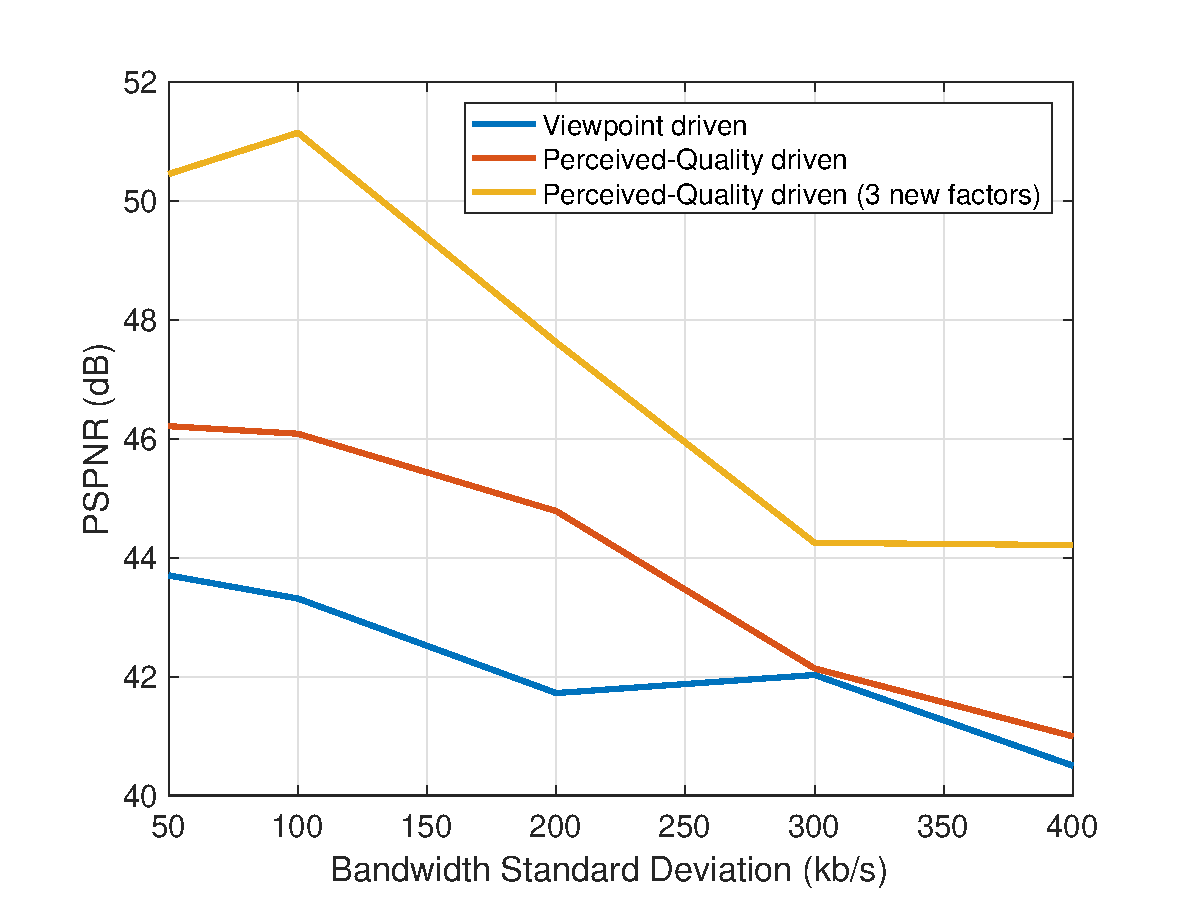
\includegraphics[width=3in]{images/throughput-PSPNR.eps}
  \caption{PSPNR of 4 methods: Viewpoint-driven, PQVRS-, PQVRS, theoretical performance.}
  \label{practical_imp}
  \end{figure}
  
    \begin{figure}
  \centering
  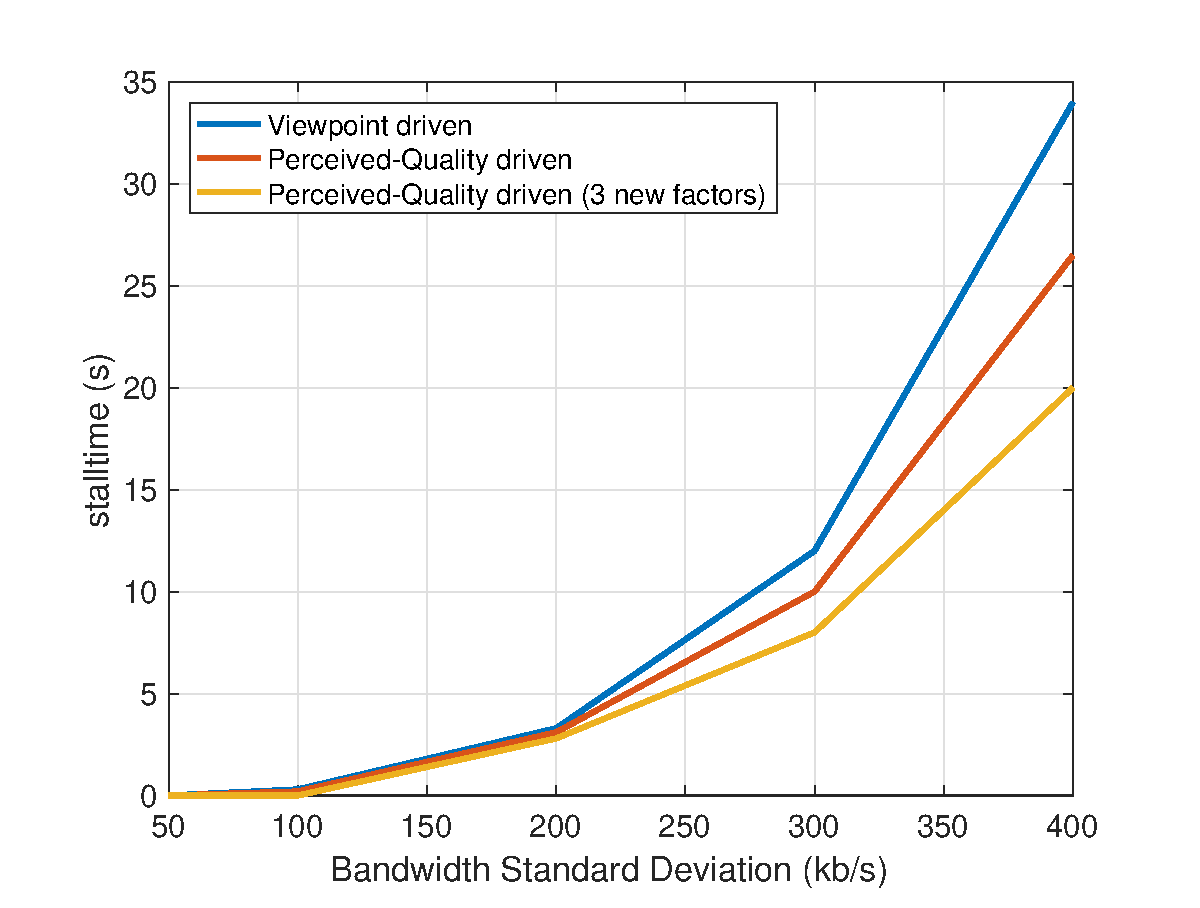
\includegraphics[width=3in]{images/throughput-stalltime.eps}
  \caption{Stalling tradeoff of 4 methods: Viewpoint-driven, PQVRS-, PQVRS, theoretical performance.}
  \label{practical_imp}
  \end{figure}

\textbf{Key observations:}

\subsection{Real-world user rating}

Based on our real-world VR streaming system, we compare above methods by real-world user rating. 

X subjects participated in the experiments. For each subject, we shown him (her) a same VR video which is streaming by Viewpoint-driven, PQVRS- and PQVRS in the same network condition. The order of display by 3 methods is random. After 3 displays, the object needs to give a rating of perceived quality for them. The rules of rating is shown in Fig. \ref{rating_rules}.

Rating rules is shown in Fig. \ref{rating_rules}. 

    \begin{figure}
  \centering
  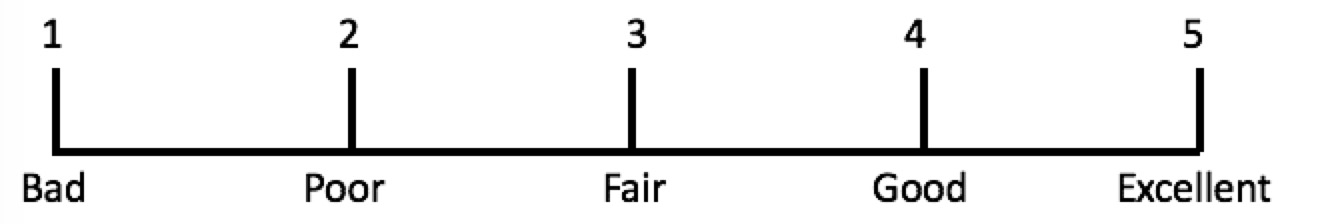
\includegraphics[width=3in]{images/rating.jpg}
  \caption{User rating rules.}
  \label{rating_rules}
  \end{figure}

Fig. \ref{rating_res} presents the result of user rating.

    \begin{figure}
  \centering
  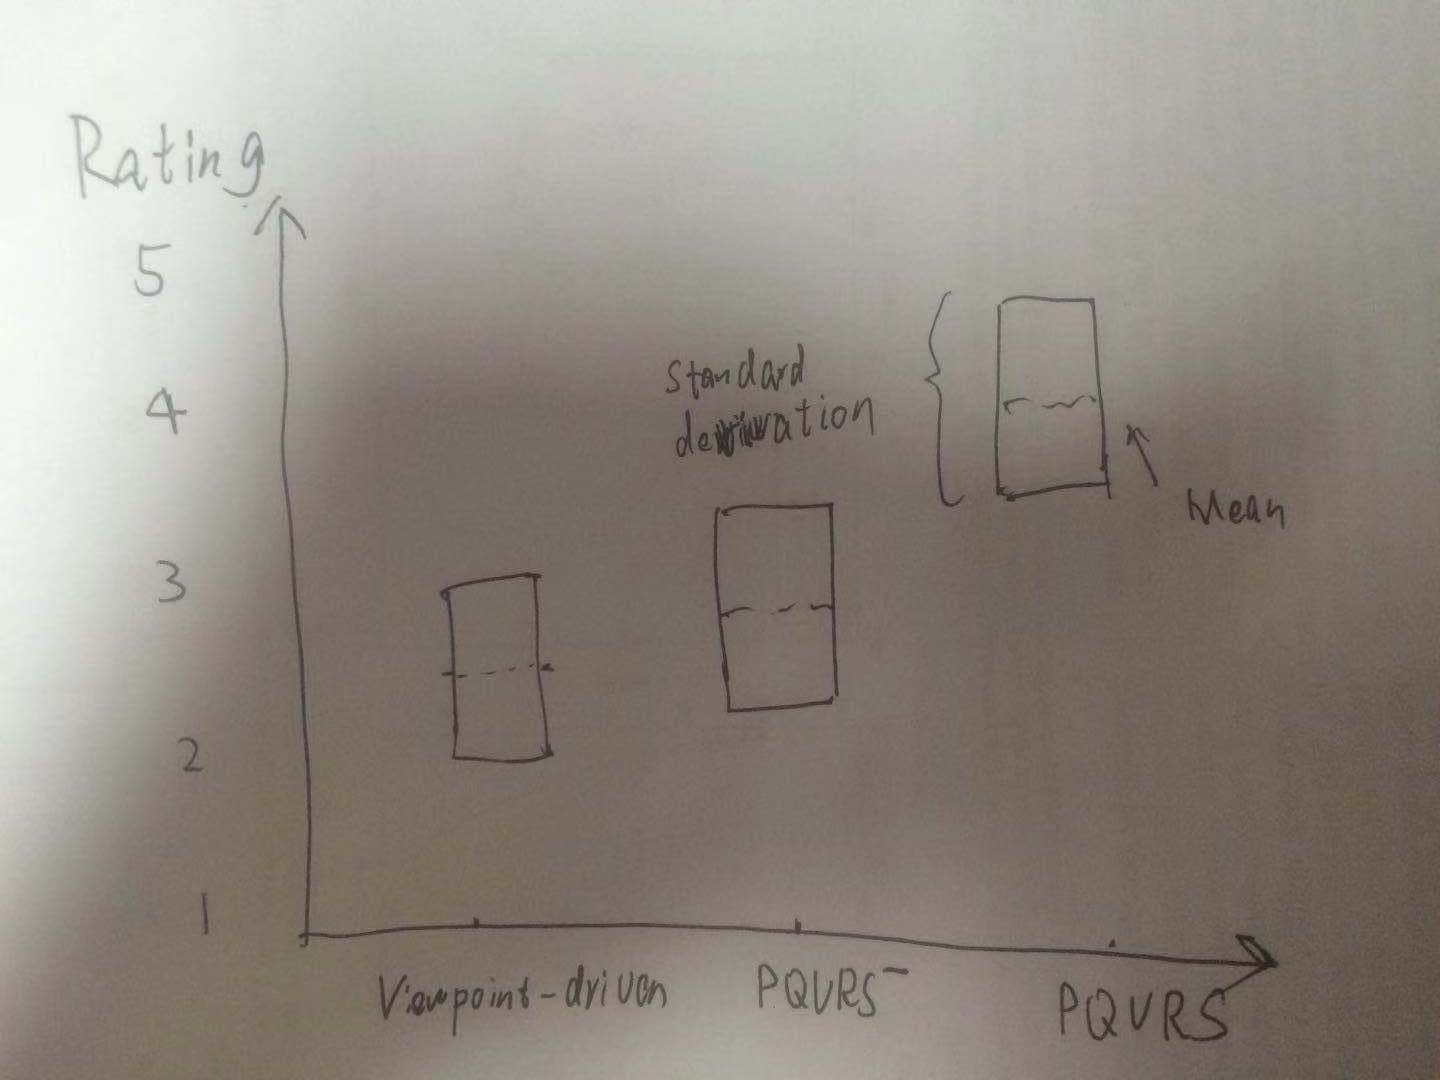
\includegraphics[width=3in]{images/rating_res.jpeg}
  \caption{User rating results.}
  \label{rating_res}
  \end{figure}

\textbf{Key observations:}

\subsection{Analysis of PQVRS improvement}

In order to clarify in which situation our proposed PQVRS has substantial improvement and in which situation it has marginal improvement, we classify our video segments according to their video types and video size.

Video types includes sports, nature, indoor, talkshow, ...

Video size is defined by the bitrate of original video. A large-size video indicates the video includes complicated or dramatically-changing content. A small-size video indicates the video includes simple and static content.

Fig. X shows the result.

    \begin{figure}
  \centering
  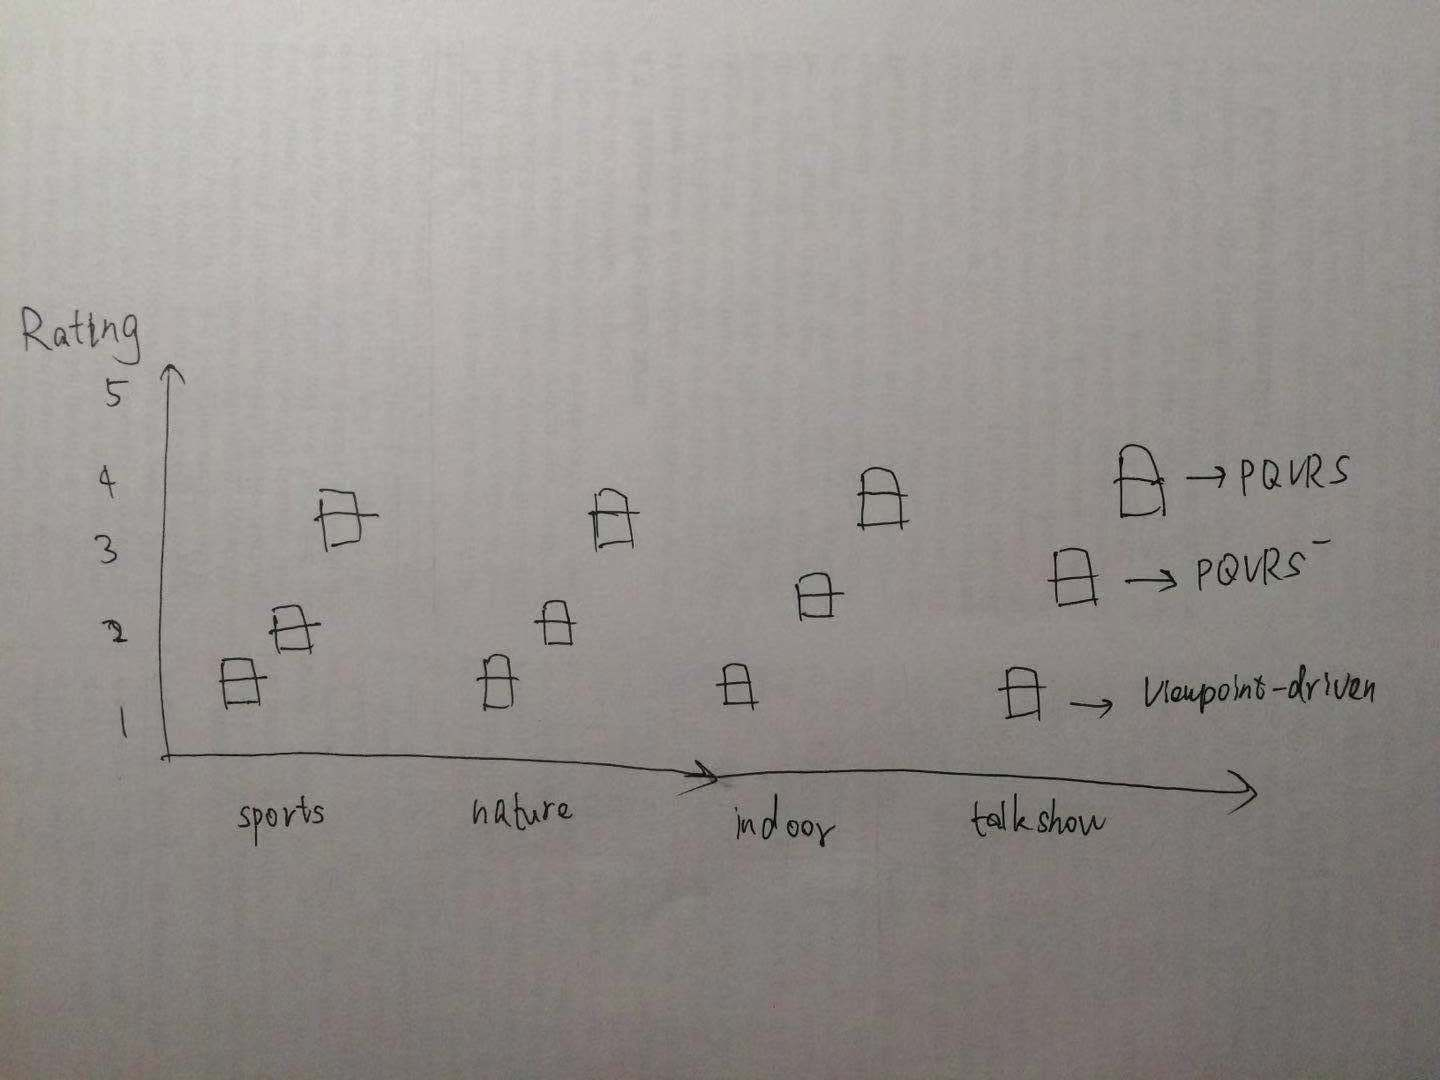
\includegraphics[width=3in]{images/rating_type.jpeg}
  \caption{User rating results for different types of videos.}
  \label{rating_res}
  \end{figure}
  
      \begin{figure}
  \centering
  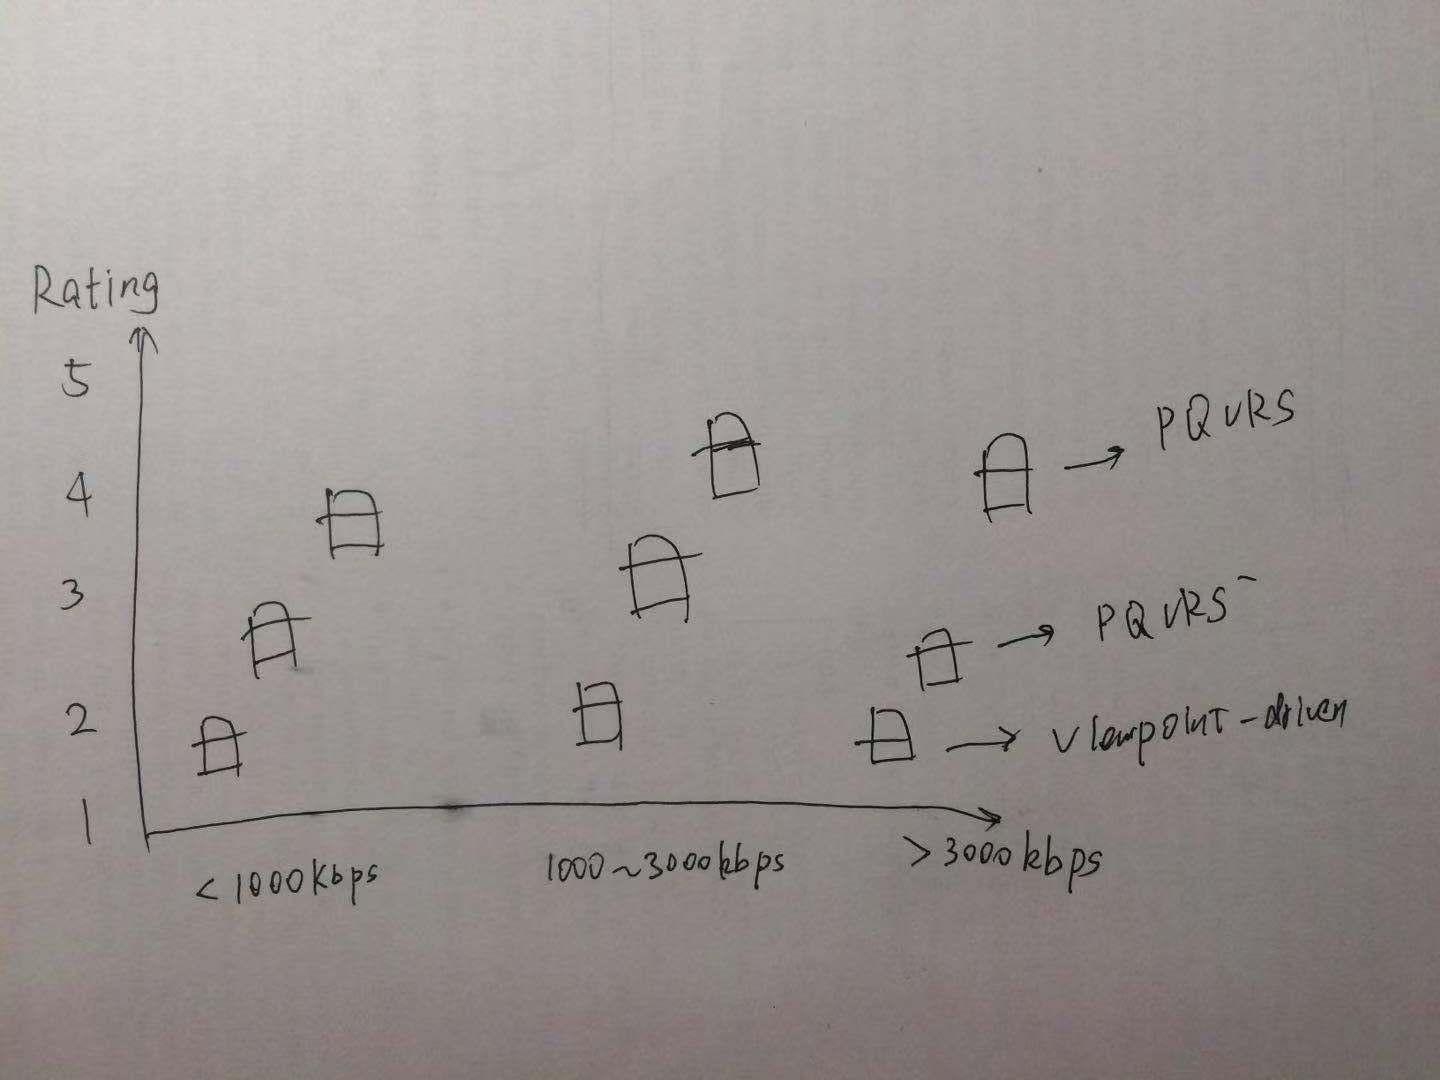
\includegraphics[width=3in]{images/rating_bitrate.jpeg}
  \caption{User rating results for videos with different original bitrate.}
  \label{rating_res}
  \end{figure}
  
\section{Related Works}

\textbf{User Perceived Quality in Video Display:}

In traditional non-VR video streaming, prior work has shown correlations between various visual characteristics and user perceived quality (e.g., users are sensitive to luminance, texture complexity, viewpoint-object distance), and built mathematical models (e.g., [] [] [] []). Our work focuses on exploring the new factors which influence user perceived quality in VR display which are never considered in traditional non-VR display, and then build an adaptive streaming system based on our insights.

\textbf{VR Adaptive Streaming:}

Monolithic streaming is the naive VR adaptive streaming method by streaming the entire 360-degree scene in constant quality without exploiting and optimizing the quality for the user’s viewport, only choose different quality for different segments.

Since user's near-future viewpoint can be predicted in high accuracy,  in order to save bandwidth, client chooses high quality for content in user's viewport and choose low quality for content out of user's viewport. There are many viewpoint-driven VR adaptive streaming works ([] [] [] [] [] ). Main difference between these adaptive streaming systems is that they choose different viewpoint prediction strategies, different rate allocation strategies, different tiling granularities and different multi-tiles decoding logics. But there are 2 common points: (1) quality allocation for each spatial part of the video is only based on the distance between content and viewpoint. (2) video is cut into tiles of equal size. Our proposed PQVRS has essential difference on these 2 points.
\section{Conclusion}

In this paper we find that in VR video display, user perceived quality is very different from video quality itself because it is related to many human visual characteristics, and optimizing perceived quality can bring out 50\% bandwidth saving.

To solve the challenges of perceived quality measurement, bandwidth efficiency problem in video tiling, and client-side perceived quality real-time computation, we build PQVRS, a real-world VR streaming system. In PQVRS, we decouple perceived quality optimization to client-side and server-side, to build a perceived quality measurement model, a server-side video tiling algorithm and a client-side perceived quality real-time computation algorithm.

Experimental results show that PQVRS saves 45\% bandwidth while providing the same perceived quality, compared with state-of-the-art VR streaming systems.



{\footnotesize \bibliographystyle{acm}
\bibliography{../common/bibliography}}

\end{document}